
\documentclass[mathserif]{beamer}%
%
%
\RequirePackage{./styles/slides}%
%
\title[%
OptimizationBenchmarking: Intro%
]{%
\mbox{\optimizationBenchmarkingText}\\%
\mbox{-- An Introduction --}%
}%
%
%
\author[Thomas Weise]{%
Thomas Weise\\%
\footnotesize{%
\mbox{\href{mailto:tweise@ustc.edu.cn}{tweise@ustc.edu.cn} $\cdot$} %
\mbox{\href{mailto:tweise@gmx.de}{tweise@gmx.de} $\cdot$} %
\mbox{\href{http://www.it-weise.de}{http://www.it-weise.de}}}}%
%
\institute[UBRI]{%
USTC-Birmingham Joint Res. Inst. in Intelligent Computation and Its Applications (UBRI)\\%
University of Science and Technology of China (USTC), Hefei 230027, Anhui, China%
}%
%
%
\begin{document}%
%
%
\startPresentation{%
\locate{}{%

\includegraphics[width=0.26\paperwidth]{graphics/barcodes/website}~\rotatebox{90}{\Large{~\textcolor{footerdarkblue}{website}}}%
\bigskip\\%

\includegraphics[width=0.26\paperwidth]{graphics/barcodes/slides}~\rotatebox{90}{\Large{~\textcolor{footerdarkblue}{slides}}}%
}{0.625}{0.16}%
}%
%
\printSectionOutlines%
%
%
%
\section{Introduction}%
%
\begin{frame}%
\frametitle{Quick Overview}%
\begin{itemize}%
\item Concept of optimization algorithms% 
\item<2-> How to \alert<4>{benchmark} optimization algorithms%
\item<3-> How to \alert<4>{evaluate data} obtained from benchmarking and how to compare algorithms
\item<4-> \alert<4>{The \optimizationBenchmarking\ Framework can help with this\only<-4>{!}}\uncover<5->{:%
\begin{itemize}%
\item It provides a graphical user interface for loading, adding meta-data (algorithm setup\dots) to, and evaluating experimental results.%
\item<6-> It can run as Docker container under Linux, MacOS, and Windows without needing \emph{any} additional software (except Docker and a browser).% 
\item<7-> It produces reports, similar to articles, in \LaTeX\ with figures and building blocks ready for use in your publications%
\end{itemize}%
}%
\end{itemize}%
\end{frame}%
%
%
\begin{frame}[t]%
\frametitle{Optimization}%
\begin{itemize}%
\item Many questions in the real world are actually optimization problems\only<2->{, e.g.,\only<-7>{%
\begin{itemize}%
%
\item \only<-5>{Find the \emph{shortest} tour for a salesman to visit certain set of cities\only<-2>{ in China and return to Hefei!}}\only<6->{\alert<6>{Traveling Salesman Problem}\scitep{ABCC2006TTSPACS,LLKS1985TTSPAGTOCO,GP2004TTSPAIV,L2011SGEFTSPIMSS}}%
%
\item<3-> \only<-5>{I need to transport $n$ items from here to another city\only<-3>{ but they are too big to transport them all at once. How can I load them best into my car so that I have to travel back and forth the least times?}}\only<6->{\alert<6>{Bin Packing Problem}\scitep{KSH1995EHFTBPP}}%
%
\item<4-> \only<-5>{Which setting of $x_1$, $x_2$, $x_3$, and $x_4$ can make $(x_1\lor\lnot x_2 \lor x_3)\land(\lnot x_2\lor\lnot x_3 \lor x_4) \land (\lnot x_1\lor\lnot x_3 \lor \lnot x_4)$ become true\only<-4>{ (or, at least, as \emph{many} of its terms as possible)?}}\only<6->{\alert<6>{Maximum (3-)Satisfiability Problem}\scitep{HS2000SAORFROS,TH2004UAIAEEFSAFSAMS,S1978TCOSP,RMK2000EASP}}%
%
\item<5-> \only<-5>{I want to build a large factory with $n$ workshops. I know the flow of material between each two workshops and now need to choose the locations of the workshops such that the overall running cost incurred by material transportation is \emph{minimized}.}\only<6->{\alert<6>{Quadratic Assignment Problem}\scitep{MF1999ACOMATSAACFTQAP,GTD1999ACOQAP}}%
\end{itemize}%
}\only<8->{ the Traveling Salesman Problem\scitep{ABCC2006TTSPACS,LLKS1985TTSPAGTOCO,GP2004TTSPAIV,L2011SGEFTSPIMSS}}%
}%
%
\item<7-> Many optimization problems are \NPHard, meaning that finding the \textcolor<9-11>{green}{best possible solution} will often take \textcolor<9-11>{green}{way too long}.%
%
\item<10-> Of course, it is easy to get \textcolor<10-11>{red}{\emph{some} solutions (usually of bad quality)}%
%
\item<11-> We use metaheuristic optimization algorithms to give us good approximate solutions within acceptable runtime.%
\item<12-> Examples of such algorithms are\only<-22>{ %
Evolutionary Algorithms\scitep{BFM1997EA,CWM2011VOEAFRWA,BFM2000EC1BAAO,BFM2000EC2BAAO,DLJD2000EC,EM1999EC,CDGDMPP1999NIIO,GT2002AIECTAA,WGOEB}\uncover<13->{, %
Ant Colony Optimization\scitep{DMC1996ACO,DS2004ACO,GM2002APBATDOP,ZBMD2004MBSFCOACS,WGOEB}\uncover<14->{, %
Evolution Strategies\scitep{R1965ES,R1973ES,R1994ES,S1965KYASDEFIDS,S1968EOEZDT1,S1975EUNO,WGOEB}\uncover<15->{, %
Differential Evolution\scitep{PSL2005DE,F2006DE,WGOEB}\uncover<16->{, %
Particle Swarm Optimization\scitep{KE1995PSO,C2006PSO,WGOEB}\uncover<17->{, %
Estimation of Distribution Algorithms\scitep{PSL2005DE,F2006DE,MMVRCC2006DE,BZSM2006DE,LZ2000DE,MM2005DE,BVPK2006DE,S2010DEFCFOAABKPARS}\uncover<18->{, %
CMA-ES\scitep{HOG1995ESAD,HO1996AANMDIESTCMA,HO2001ESCMA,HMK2003RTTCOTDESWCMACE,HK2004ETCESOMTF,H2006TCESACR,AH2005ARCESWIPS,AH2005PEOAALSEA}\uncover<19->{, and %
Local Search methods\scitep{HS2005SLSFAA,AL1997LSICO,DBSD2001DOILSA}\uncover<20->{ such as %
Simulated Annealing\scitep{SSF2002FCAIFSA,LA1987SATAA,B1987GAASA,JCS2003HC,KGV1983SA,VC1985SA,DPSW1982MCTICO,DPSW1982MCTICO2,P1970AMCMFTASOCTOCOP,WGOEB}\uncover<21->{ or %
Tabu Search\scitep{G1989TSPI,G1990TSPII,GL1993TABU,DWH1989TSTATAAATNN,BT1994TABU}\uncover<22->{, %
as well as hybrids of local and global search, such as Memetic Algorithms\scitep{M1989MA,M2002MA,MC2003AGITMA,ES2003HWOTMA,HKS2005RAIMA,DM2004MA,RS1994FMA}%
}}}}}}}}}}}\only<23->{\dots\ \alert{many}}%
%
\item<24-> \alert<24>{Which of them is best (for my problem)?}%
\item<25-> \alert<25>{How can I make a good algorithm better (for my problem)?}%
%
\end{itemize}%
~\\~\\~\\~\\~\\~\\~\\~\\~\\~\\~\\~\\~\\~\\~\\~\\~\\~\\~\\~\\~\\~\\~\\~\\~\\~\\~\\~\\~\\~\\~\\~\\~\\%
%
\locateGraphic{2}{width=0.6\paperwidth}{graphics/problem_examples/tsp/tsp}{0.2}{0.29}%
\locateGraphic{3}{width=0.875\paperwidth}{graphics/problem_examples/bin_packing/bin_packing}{0.0625}{0.495}%
\locateGraphic{4}{width=0.55\paperwidth}{graphics/problem_examples/sat/sat}{0.225}{0.5}%
\locateGraphic{5}{width=0.85\paperwidth}{graphics/problem_examples/qap/qap}{0.075}{0.625}%
\locateGraphic{7}{width=0.75\paperwidth}{graphics/exponential_functions/exponential_functions}{0.1625}{0.55}%
%
\locateGraphic{8}{width=0.75\paperwidth}{graphics/optimization_concept/optimization_concept_1}{0.125}{0.53}%
\locateGraphic{9}{width=0.75\paperwidth}{graphics/optimization_concept/optimization_concept_2}{0.125}{0.53}%
\locateGraphic{10}{width=0.75\paperwidth}{graphics/optimization_concept/optimization_concept_3}{0.125}{0.53}%
\locateGraphic{11}{width=0.75\paperwidth}{graphics/optimization_concept/optimization_concept}{0.125}{0.53}%
%
\end{frame}%
%
%
\begin{frame}[t]%
\frametitle{Performance and Anytime Algorithms}%
%
\emph{\inQuotes{We use metaheuristic optimization algorithms to give us \alert<3->{good approximate solutions} within \alert<4->{acceptable runtime}.}}%
%
\uncover<2->{%
\begin{itemize}%
\item Algorithm performance has two dimensions\scitep{NAFR2010RPBBOB2ES,WCTLTCMY2014BOAAOSFFTTSP}:\uncover<3->{ solution quality\uncover<4->{ and required runtime}}%
\only<-9>{%
\item<5-> Anytime Algorithms\scitep{BD1989STDPP2} are optimization methods which maintain an approximate solution at \emph{any time} during their run and iteratively improve this guess.%
\item<6-> All metaheuristics are Anytime Algorithms.%
\item<7-> Several exact methods like Branch-and-Bound\scitep{LMSK1963AAFTTSP,Z1993TBABACSOTATSP,Z1999TAADFBABACSOTATSP} are Anytime Algorithms.%
\item<8-> Consequence: Most optimization algorithms produce approximate solutions of different qualities at different points during their process.%
\item<9-> \alert{Experiments must capture data on the whole runtime behavior!}%
}%
\item<10-> If we just compare \inQuotes{final} results, we may arrive at incomplete \only<12->{or entirely wrong} conclusions%
\end{itemize}%
}%
%
\locateGraphic{3}{width=0.55\paperwidth}{graphics/performance/performance_dimensions/performance_dimensions_1}{0.225}{0.542}%
\locateGraphic{4}{width=0.55\paperwidth}{graphics/performance/performance_dimensions/performance_dimensions_2}{0.225}{0.542}%
\locateGraphic{5,10}{width=0.55\paperwidth}{graphics/performance/performance_dimensions/performance_dimensions}{0.225}{0.542}%
\locateGraphic{11}{width=0.55\paperwidth}{graphics/performance/performance_dimensions/performance_cuts}{0.225}{0.542}%
\locateGraphic{12}{width=0.55\paperwidth}{graphics/problems_with_points/points}{0.225}{0.542}%
\locateGraphic{13}{width=0.55\paperwidth}{graphics/problems_with_points/lines}{0.225}{0.542}%
%
\end{frame}%
%
%
\begin{frame}[t]%
\frametitle{Experimentation Procedure}%
\begin{itemize}%
\item The following experimentation procedure is suitable for optimization and Machine Learning\uncover<2->{:%
\begin{enumerate}%
\item Select a set of (well-known) benchmark instances which covers some \textcolor<18>{red}{different problem features}\only<-11>{ \alert{(done)}}\only<3-4>{:%
\begin{itemize}%
%
\only<-3>{%
\item<3-> e.g., \tspLib\expandafter\scitep{\tspLibReferences} for the TSP has instances with different numbers of cities and geometries%
}%
\only<-4>{%
\item<4-> e.g., \bbob\expandafter\scitep{\bbobReferences} offers different benchmark functions for numerical optimization problems%
}%
%
\end{itemize}%
}%
\item<5-> Do experiments\only<11->{ with \textcolor<18>{red}{different algorithms/setups}\only<-11>{ \alert{(done)}}}\only<6-10>{:%
\begin{itemize}%
\item several independent runs of algorithm for each benchmark instance%
\item<7-> collect algorithm progress information, e.g., as \emph{\inQuotes{(runtime, best-objective-value-so-far)}} tuples%
\item<8-> one log file per run, each log file has several such tuples%
\item<9-> repeat for different algorithm parameter settings (e.g., different population sizes of an EA)%
\item<10-> repeat with other algorithms for comparison purposes%
\end{itemize}%
}%
\item<12-> Evaluate the gathered data\only<13->{, e.g.:%
\begin{itemize}%
\item \textcolor<17>{green}{draw diagrams of progress of solution quality over time}%
\item<14-> \textcolor<17>{green}{draw diagrams of advanced statistical parameters such as ECDF\scitep{HAFR2012RPBBOBES,HS1998ELVAPAR,TH2004UAIAEEFSAFSAMS,WCTLTCMY2014BOAAOSFFTTSP}\only<15->{ and ERT\scitep{HAFR2012RPBBOBES,WCTLTCMY2014BOAAOSFFTTSP}} (over time)}%
\end{itemize}%
}%
%
\item<16-> But doing this is cumbersome\dots%
\end{enumerate}%
}%
\item<17-> The \optimizationBenchmarking\ framework \textcolor<17>{green}{can automatize} much of the evaluation procedure\uncover<18>{\dots}%
\item<18-> {\dots}and make use of \textcolor<18>{red}{meta-data} about experiments to group and aggregate information.% 
\end{itemize}%
%
\locateWithCaption{3}{%
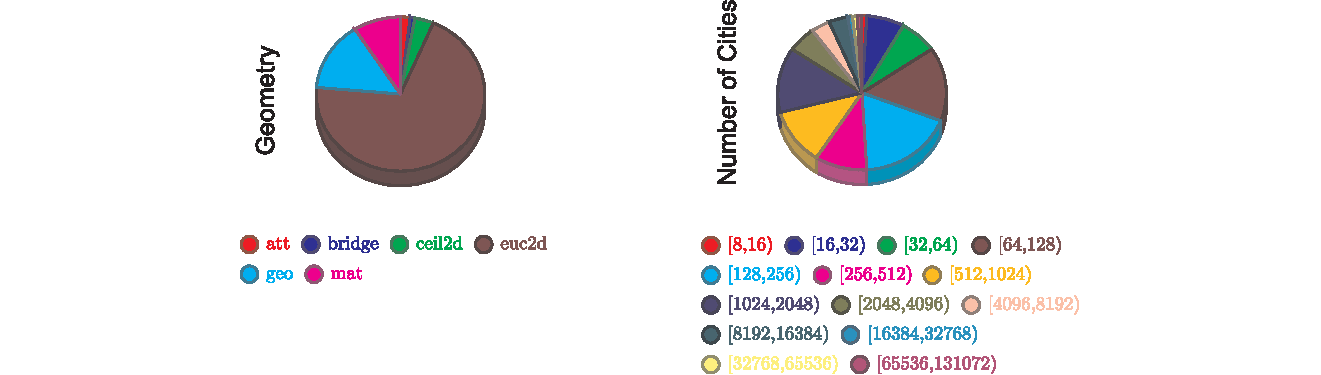
\includegraphics[width=0.925\paperwidth]{graphics/tspLib_features/tspLib_features_symmetric}%
}{%
The relative amounts of the instances of the 110 symmetric instances of \tspLib\expandafter\scitep{\tspLibReferences} according to their features (the 10 asymmetric instances are not plotted).%
}{0.0375}{0.51}{0.925}%
%
\locateWithCaption{4}{%
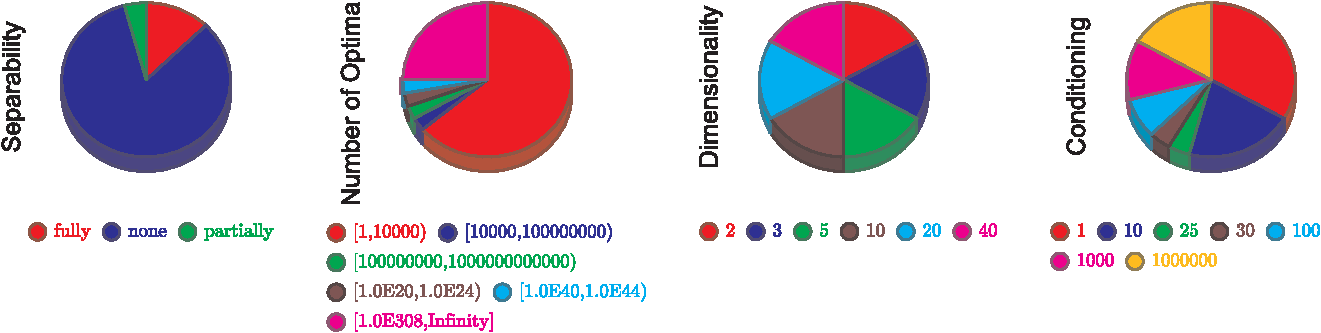
\includegraphics[width=0.925\paperwidth]{graphics/bbob_features/bbob_features}%
}{%
The relative amounts of \bbob\expandafter\scitep{\bbobReferences} benchmark functions according to their features.%
}{0.0375}{0.51}{0.925}%
%
\locateWithCaption{7-8}{%
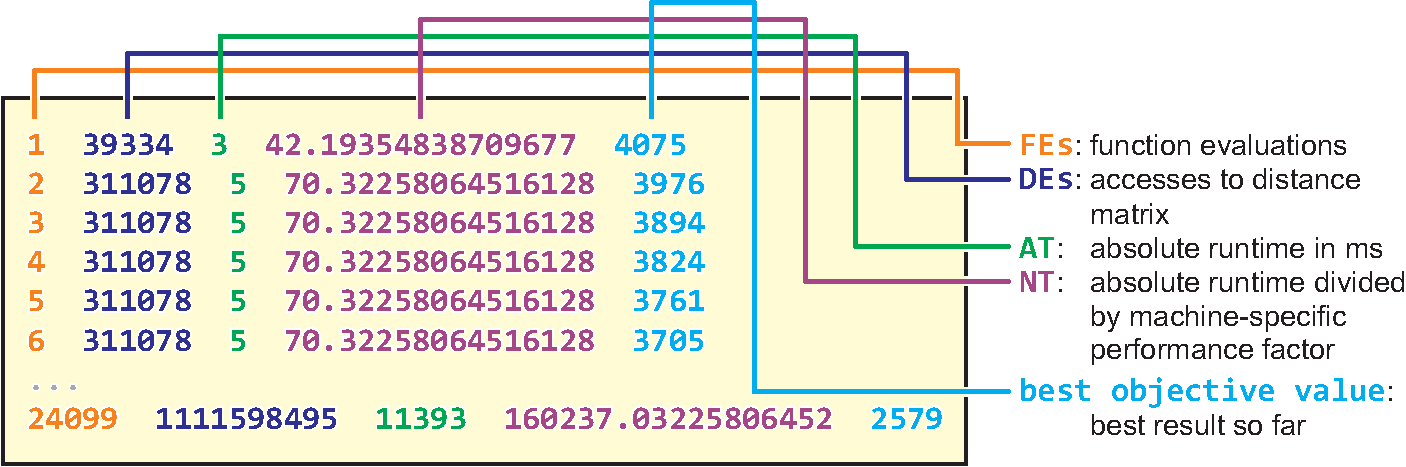
\includegraphics[width=0.8\paperwidth]{graphics/tspSuite_logfile_example/tspSuite_logfile_example}%
}{%
Example for data collected in a log file by \tspSuite\expandafter\scitep{\tspSuiteReferences}.%
}{0.0375}{0.53}{0.925}%
%
\locateWithCaption{13-15}{
\strut%
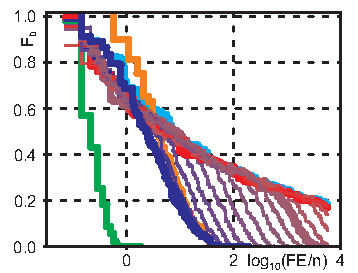
\includegraphics[width=0.28\paperwidth]{graphics/performance/progress_example/progress_example}%
\uncover<14->{%
\strut\hfill\strut%
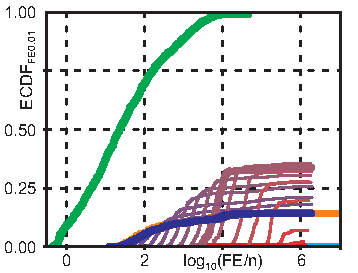
\includegraphics[width=0.28\paperwidth]{graphics/performance/ecdf_example/ecdf_example}%
\uncover<15->{%
\strut\hfill\strut%
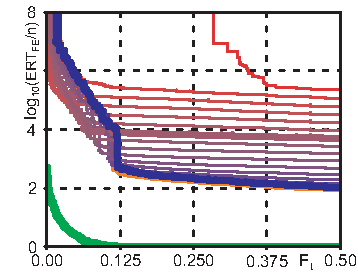
\includegraphics[width=0.28\paperwidth]{graphics/performance/ert_example/ert_example}%
}}\strut%
}{%
Examples for progress\only<14->{ and ECDF}\only<15->{, ERT, and ECDF} diagrams from \tspSuite\expandafter\scitep{\tspSuiteReferences} for different algorithms (signified by different colors) over different sub-sets of the \tspLib\expandafter\scitep{\tspLibReferences} data.%
}{0.0375}{0.545}{0.925}%
%
\end{frame}%%
%
\section{Installation}%
%
\begin{frame}[t]%
\frametitle{Installation}%
\centering\footnotesize%
%
\strut\vfill%
\mbox{\textbf{\large{Website:~\href{http://optimizationbenchmarking.github.io}{http://optimizationbenchmarking.github.io}}}}%
\vfill%
%
\begin{itemize}%
%
\item Stand-Alone GUI: easily store, annotate, and process your experimental results:%
\begin{itemize}%
\item client/server application: computation at the server, joint repository for data of your group%
\item software requirements: Java~7~JDK\scitep{JAVA2PSESAS}, TeX~Live\scitep{TEXLIVE}, \codeil{R}\scitep{WU2006TRPFSC} with several packages%
\item download software from web page%
\item \mbox{\codeil{java -jar evaluatorGui.jar}}%
\item open browser to \codeil{localhost}%
\end{itemize}%
%
\vfill\vfill%
%
\item Application Dockerized for you!%
\begin{itemize}%
\item install Docker from\\\url{http://www.docker.com/} and do%
\item \mbox{\codeil{docker run -t -i -p 80:8080/tcp}} \mbox{\codeil{optimizationbenchmarking/evaluator-gui}}%
\item open browser to \codeil{localhost}%
\end{itemize}%
%
\vfill%
%
\locateGraphic{}{width=0.37\paperwidth}{graphics/website/website}{0.61}{0.437}%
%
\end{itemize}%
%
\end{frame}%
%

%
%
\edef\maxSat{MAX-SAT}%
\edef\maxTSat{MAX-3SAT}%
\def\oFlip{\ensuremath{1}-flip}%
\def\tFlip{\ensuremath{2}-flip}%
\def\mFlip{\ensuremath{m}-flip}%
%
\gdef\maxSatClauses{\textcolor{blue}{\ensuremath{k}}}%
\gdef\maxSatVariables{\textcolor{green}{\ensuremath{n}}}%
\gdef\maxSatVariable{\ensuremath{x}}%
\gdef\maxSatVariablei#1{\ensuremath{\maxSatVariable_{#1}}}%
\gdef\maxSatFormula{\ensuremath{B}}%
%
\section{Example: \maxSat}%
%
%%
\begin{frame}[t]%
\frametitle{\maxSat}%
\begin{itemize}%
\item \only<8->{Maximum }Satisfiability Problems (SAT)\only<-7>{\scitep{HS2000SAORFROS}}\only<8->{\scitep{HS2005SLSFAA}}\uncover<2->{:%
\begin{itemize}
\item Given: Formula \maxSatFormula\ in Boolean logic%
\uncover<3->{ with \maxSatVariables\ Boolean variables $\vec{\maxSatVariable}=(\maxSatVariablei{1}, \maxSatVariablei{2},\dots, \maxSatVariablei{\maxSatVariables})$%
\uncover<4->{, which appear either directly or negated%
\uncover<5->{ in \maxSatClauses\ \inQuotes{\texttt{or}} clauses%
\uncover<6->{, which are all combined with into one \inQuotes{\texttt{and}}}}}}%
\item<7-> \only<-7>{SAT Goal: find a setting for these variables so that $\maxSatFormula$ becomes \texttt{true}}%
\only<8->{\maxSat\ Goal\scitep{HS2005SLSFAA}: minimize objective function $\objectiveFunctionb{\vec{x}} = \textnormal{number of clauses which are \texttt{false}}$.}%
\item<9-> $\objectiveFunctionb{\vec{x}}=0$ $\Longrightarrow$ all clauses are \texttt{true}, SAT problem solved%
\end{itemize}%
}%
%%
\item<10-> We want to compare the performance of \textcolor<10-11,14->{red}{six different} (trivial) \textcolor<10-11,14->{red}{algorithm setups}\only  <12->{ differing in two parameters}\uncover<11->{:%
\begin{enumerate}%
\item \textcolor<12>{orange}{\oFlip} Hill Climber \textcolor<13>{orange}{without Restarts}%
\item \textcolor<12>{orange}{\oFlip} Hill Climber \textcolor<13>{cyan}{with Restarts}%
\item \textcolor<12>{violet}{\tFlip} Hill Climber \textcolor<13>{orange}{without Restarts}%
\item \textcolor<12>{violet}{\tFlip} Hill Climber \textcolor<13>{cyan}{with Restarts}%
\item \textcolor<12>{cyan}{\mFlip} Hill Climber \textcolor<13>{orange}{without Restarts}%
\item \textcolor<12>{cyan}{\mFlip} Hill Climber \textcolor<13>{cyan}{with Restarts}%
\end{enumerate}%
%
\only<12>{\smallskip%
\small{%
\textcolor<12>{orange}{\oFlip}: one variable flipped in the current solution at each step, %
\textcolor<12>{violet}{\tFlip}: two variables flipped, %
\textcolor<12>{cyan}{\mFlip}: number $m$ of variables to flip chosen according to geometric distribution%
}}%
%
\only<13>{\smallskip%
\small{%
\textcolor<13>{cyan}{with Restarts}: if no improvement for $z$ steps, restart and set $z=z+1$, initially $z=1$, %
\textcolor<13>{orange}{without Restarts}: doesn't do this%
}}}%
%
\item<14-> We investigate the algorithms on $10\times 10$ (simple) instances from \satLib\expandafter\scitep{\satLibReferences} with \textcolor{red}{ten different values of \maxSatVariables} from 20 to 250 (\maxSatClauses\ is fixed for each value of \maxSatVariables)
%
\end{itemize}%
%
\locateGraphic{-2,7-9}{width=0.55\paperwidth}{graphics/problem_examples/sat/sat}{0.225}{0.54}%
\locateGraphic{3}{width=0.55\paperwidth}{graphics/problem_examples/sat/sat_variables}{0.225}{0.54}%
\locateGraphic{4}{width=0.55\paperwidth}{graphics/problem_examples/sat/sat_negation}{0.225}{0.54}%
\locateGraphic{5}{width=0.55\paperwidth}{graphics/problem_examples/sat/sat_or}{0.225}{0.54}%
\locateGraphic{6}{width=0.55\paperwidth}{graphics/problem_examples/sat/sat_and}{0.225}{0.54}%
%
\end{frame}%
%
%
\begin{frame}[t]%
\frametitle{Example of Log File}%
%
\begin{itemize}%
\only<-1>{\item Now we do experiments and collect data.}%
\item<2-> Example log file obtained from applying the 2-flip Hill Climber with Restarts to the 2\textsuperscript{nd} benchmark instance of set \texttt{uf075}.%
\end{itemize}%
%
\begin{locateBox}[2-]{0.25}{0.235}
\begin{listingBlock}[0.65]{Log File \texttt{uf075-02\_2FlipHCrs\_01.txt}.}
\centering
\begin{scaledBox}{!}{0.3\paperheight}
\lstinputlisting[tabsize=17]{graphics/maxsat_example/exampleMaxSatLogFile.txt}
\end{scaledBox}
\end{listingBlock}
\end{locateBox}
%
\begin{locateBox}[3-]{0}{0}
\begin{pgfpicture}%
\pgfpathrectangle{\pgfpoint{0pt}{0pt}}{\pgfpoint{\paperwidth}{\paperheight}}%
\pgfusepath{use as bounding box,clip}%
%
\pgfsetcolor{blue}%
\pgftext[right,bottom,at=\pgfpoint{0.2\paperwidth}{0.55\paperheight}]{log point}%
\pgfsetlinewidth{1pt}%
\pgfpathmoveto{\pgfpoint{0.21\paperwidth}{0.56\paperheight}}%
\pgfpathlineto{\pgfpoint{0.32\paperwidth}{0.525\paperheight}}%
\pgfusepath{stroke}%
\pgfsetlinewidth{2pt}%
\pgfpathrectangle{\pgfpoint{0.32\paperwidth}{0.51\paperheight}}{\pgfpoint{0.52\paperwidth}{0.03\paperheight}}%
\pgfusepath{stroke}%
%
\uncover<4->{%
%
\pgfsetcolor{red}%
\pgftext[right,bottom,at=\pgfpoint{0.2\paperwidth}{0.45\paperheight}]{ellapsed \measureFEs}%
\pgfsetlinewidth{1pt}%
\pgfpathmoveto{\pgfpoint{0.21\paperwidth}{0.46\paperheight}}%
\pgfpathlineto{\pgfpoint{0.36\paperwidth}{0.4\paperheight}}%
\pgfusepath{stroke}%
\pgfsetlinewidth{2pt}%
\pgfpathrectangle{\pgfpoint{0.36\paperwidth}{0.085\paperheight}}{\pgfpoint{0.1\paperwidth}{0.585\paperheight}}%
\pgfusepath{stroke}%
%
\uncover<5->{%
\pgfsetcolor{green}%
\pgftext[right,bottom,at=\pgfpoint{0.2\paperwidth}{0.35\paperheight}]{runtime [\nano\second]}%
\pgfsetlinewidth{1pt}%
\pgfpathmoveto{\pgfpoint{0.21\paperwidth}{0.365\paperheight}}%
\pgfpathlineto{\pgfpoint{0.56\paperwidth}{0.3\paperheight}}%
\pgfusepath{stroke}%
\pgfsetlinewidth{2pt}%
\pgfpathrectangle{\pgfpoint{0.56\paperwidth}{0.085\paperheight}}{\pgfpoint{0.11\paperwidth}{0.585\paperheight}}%
\pgfusepath{stroke}%
%
\uncover<6->{%
\pgfsetcolor{violet}%
\pgftext[right,bottom,at=\pgfpoint{0.2\paperwidth}{0.25\paperheight}]{\measureObjectiveValue: best \objectiveFunctionb{\vec{x}}}%
\pgfsetlinewidth{1pt}%
\pgfpathmoveto{\pgfpoint{0.21\paperwidth}{0.26\paperheight}}%
\pgfpathlineto{\pgfpoint{0.7\paperwidth}{0.2\paperheight}}%
\pgfusepath{stroke}%
\pgfsetlinewidth{2pt}%
\pgfpathrectangle{\pgfpoint{0.7\paperwidth}{0.085\paperheight}}{\pgfpoint{0.1\paperwidth}{0.585\paperheight}}%
\pgfusepath{stroke}%
}}}%
\end{pgfpicture}%
\end{locateBox}%
%
\end{frame}
%
\begin{frame}[t]{Obtained Data}%
\def\shortcutForAfterExperimentText{$6*20*10*10=\numprint{12000}$ log files\only<-6>{!}\uncover<7->{ (with $\numprint{607993}$ log points and $8.6~\mebi\byte$ in total)!}}%
\parbox[t]{0.6\paperwidth}{%
\bigskip%
\begin{itemize}%
\item OK, so after the experiment\only<-7>{\dots%
\uncover<2->{%
\begin{itemize}%
\item {\dots}we have $20$ independent runs (log files)%
\item<3-> for each of the $6$ algorithm setups,%
\item<4-> on each of the $10$ benchmark instances%
\item<5-> of each of the $10$ instance sets\uncover<6->{, i.e.,}%
\item<6-> \shortcutForAfterExperimentText%
\end{itemize}%
}%
}%
\only<8->{ we have \shortcutForAfterExperimentText}%
\item<9-> \alert<-12>{How can we extract useful information from them\only<-8>{?}%
\uncover<10->{ in order to answer the questions which algorithm performs best, when, and why?}%
\uncover<11->{ What is the impact of the benchmark feature \maxSatVariables\ on the performance?}%
\uncover<12->{ What is the impact of the search operator and the restarts on the performance?}}%
\item<13-> What you most likely do: Write your own small program.%
\item<14-> What you now can do: Use our \optimizationBenchmarking\ evaluator!%
\end{itemize}%
}%
%
\locate{2-}{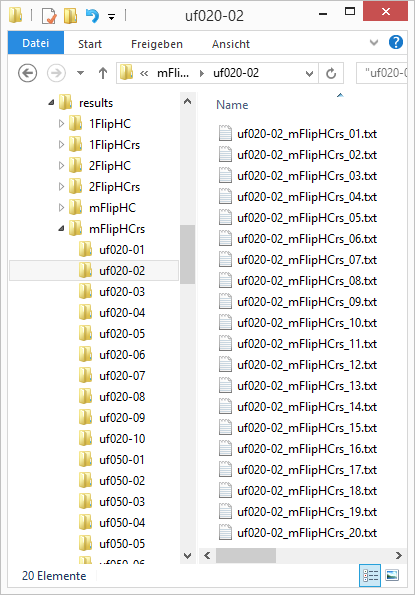
\includegraphics[width=0.33\paperwidth]{graphics/maxsat_example/maxsat_example_log_file_folder_structure}}{0.65}{0.21}%
%
\begin{locateBox}[2-5]{0.65}{0.21}
\begin{pgfpicture}%
\pgfpathrectangle{\pgfpoint{0pt}{0pt}}{\pgfpoint{0.33\paperwidth}{0.79\paperheight}}%
\pgfusepath{use as bounding box,clip}%
%
\pgfsetcolor{alert}%
\pgfsetlinewidth{0.5pt}%
%
\only<3>{%
\pgfpathrectangle{\pgfpoint{0.05\paperwidth}{0.649\paperheight}}{\pgfpoint{0.07\paperwidth}{0.02\paperheight}}%
\pgfpathrectangle{\pgfpoint{0.05\paperwidth}{0.626\paperheight}}{\pgfpoint{0.07\paperwidth}{0.02\paperheight}}%
\pgfpathrectangle{\pgfpoint{0.05\paperwidth}{0.603\paperheight}}{\pgfpoint{0.07\paperwidth}{0.02\paperheight}}%
\pgfpathrectangle{\pgfpoint{0.05\paperwidth}{0.580\paperheight}}{\pgfpoint{0.07\paperwidth}{0.02\paperheight}}%
\pgfpathrectangle{\pgfpoint{0.05\paperwidth}{0.557\paperheight}}{\pgfpoint{0.07\paperwidth}{0.02\paperheight}}%
\pgfpathrectangle{\pgfpoint{0.05\paperwidth}{0.534\paperheight}}{\pgfpoint{0.07\paperwidth}{0.02\paperheight}}%
}%
%
\only<2>{%
\pgfpathrectangle{\pgfpoint{0.272\paperwidth}{0.21\paperheight}}{\pgfpoint{0.018\paperwidth}{0.445\paperheight}}%
\pgfpathrectangle{\pgfpoint{0.013\paperwidth}{0.17\paperheight}}{\pgfpoint{0.06\paperwidth}{0.02\paperheight}}%
}%
%
\only<4>{%
\pgfpathrectangle{\pgfpoint{0.06\paperwidth}{0.319\paperheight}}{\pgfpoint{0.06\paperwidth}{0.212\paperheight}}%
}%
%
\only<5>{%
\pgfpathrectangle{\pgfpoint{0.06\paperwidth}{0.513\paperheight}}{\pgfpoint{0.0433\paperwidth}{0.02\paperheight}}%
\pgfpathrectangle{\pgfpoint{0.06\paperwidth}{0.2958\paperheight}}{\pgfpoint{0.0433\paperwidth}{0.02\paperheight}}%
}%
%
\pgfusepath{stroke}%
%
\end{pgfpicture}%
\end{locateBox}%
\end{frame}%
%
\begin{frame}[label=maxSatInteractiveDemoStart]%
\frametitle{Demo}%
\centering\alert{\textbf{\LARGE{Demo}}}%
\bigskip%
\begin{itemize}%
\item the evaluator GUI%
\item the structure of the data%
\item running an evaluation process%
\item viewing the results%
\end{itemize}%
\bigskip%
\centering\scalebox{1.8}{\hyperlink{maxSatDemoStart}{\beamergotobutton{go to static demo slides}}}%
\locateGraphic{}{width=0.2\paperwidth}{graphics/logo/logo}{0.725}{0.65}%
\end{frame}%
%
%
\begin{frame}[b,label=maxSatInteractiveDemoEnd]%
\frametitle{The Flow}%
%
\only<-1>{%
\strut\vfill\strut%
\centering{\LARGE{\textbf{\alert{The evaluator works as follows\dots}}}}%
\strut\vfill\strut%
}%
%
\locate{2-3}{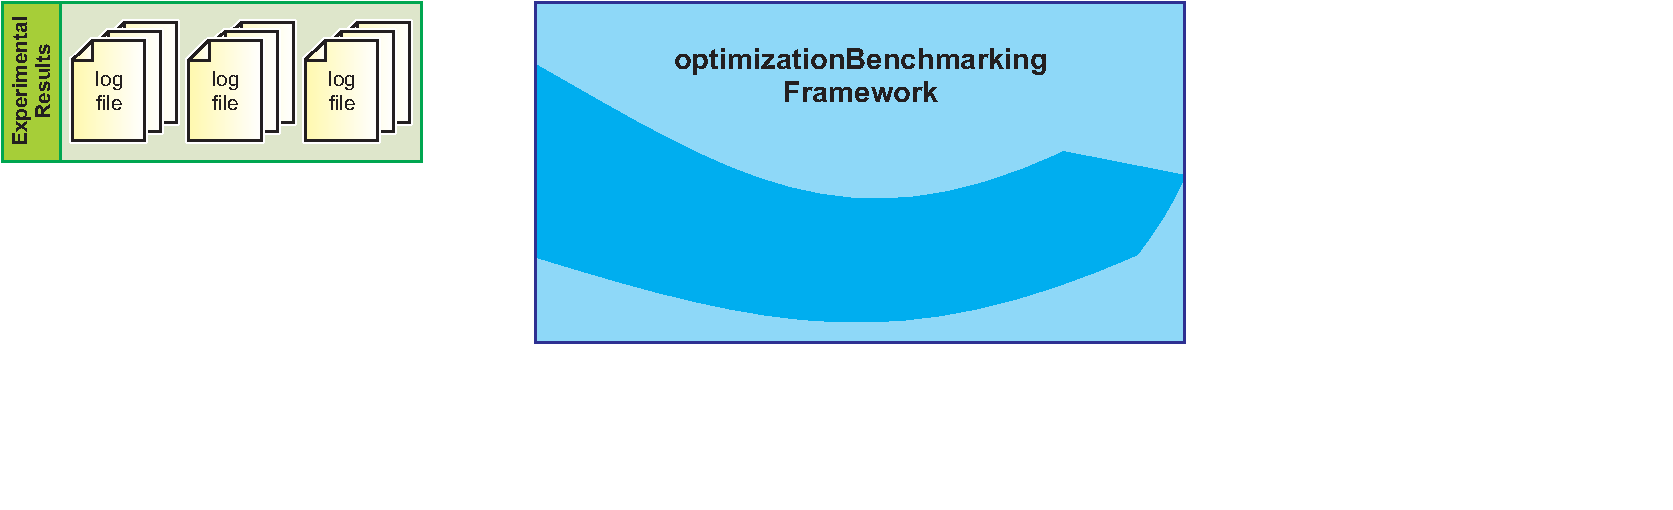
\includegraphics[width=0.9\paperwidth]{graphics/flow/flow_input_1_results}}{0.05}{0.16}%
\locate{4-5}{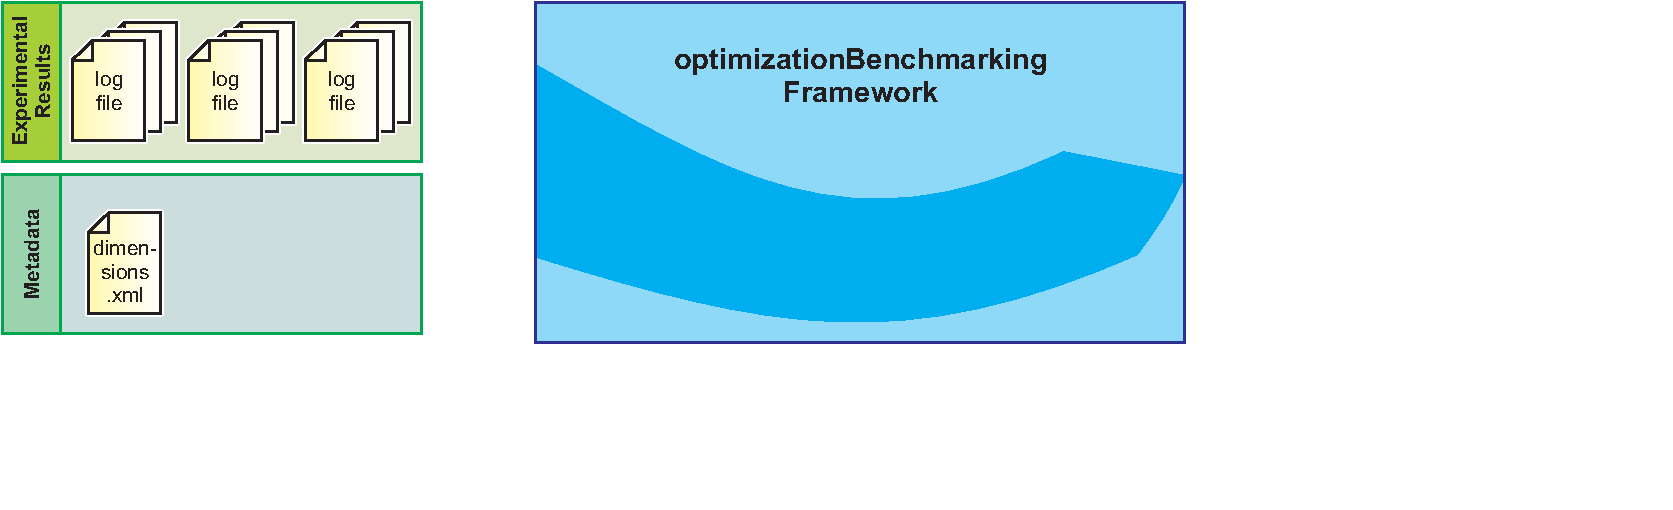
\includegraphics[width=0.9\paperwidth]{graphics/flow/flow_input_2_dimensions}}{0.05}{0.16}%
\locate{6-7}{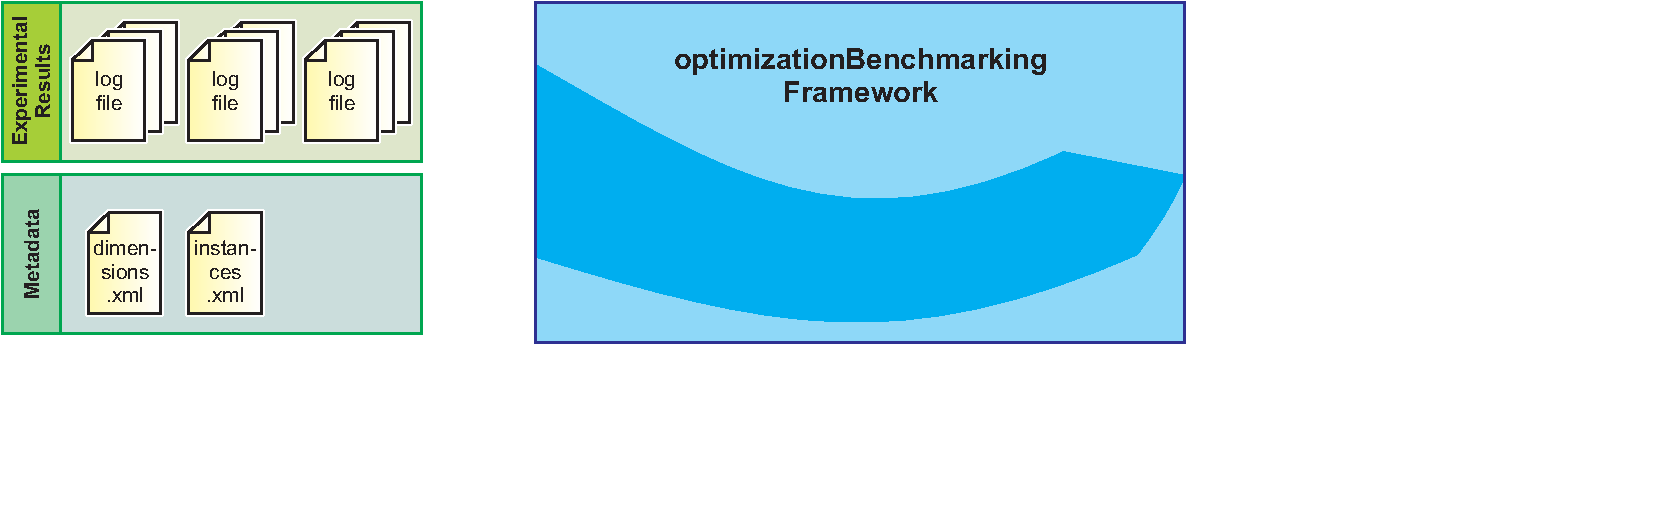
\includegraphics[width=0.9\paperwidth]{graphics/flow/flow_input_3_instances}}{0.05}{0.16}%
\locate{8-9}{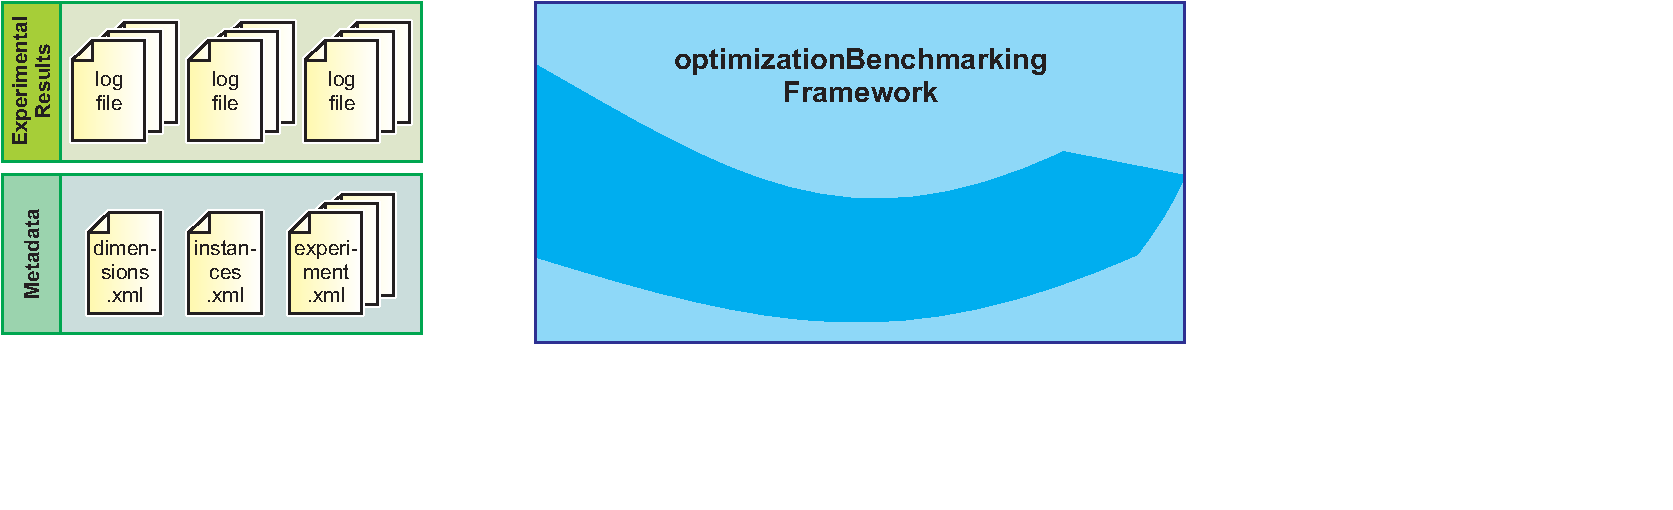
\includegraphics[width=0.9\paperwidth]{graphics/flow/flow_input_4_experiment}}{0.05}{0.16}%
\locate{10-11}{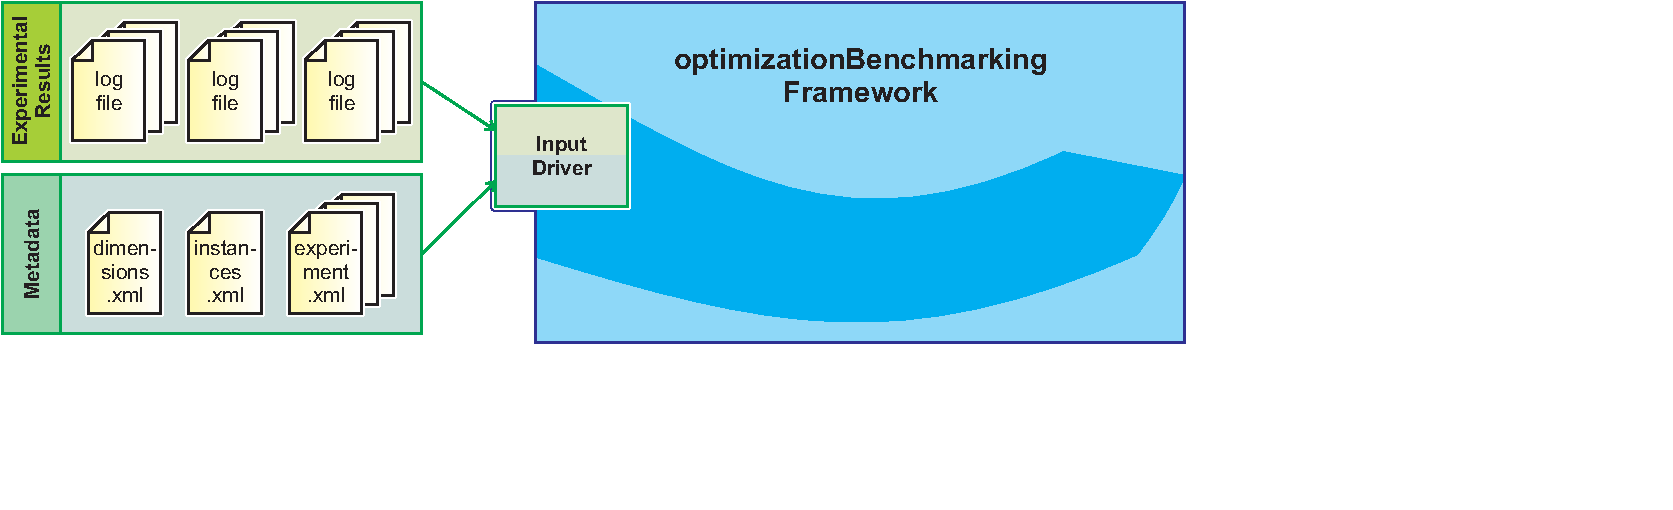
\includegraphics[width=0.9\paperwidth]{graphics/flow/flow_input_5_driver}}{0.05}{0.16}%
\locate{12}{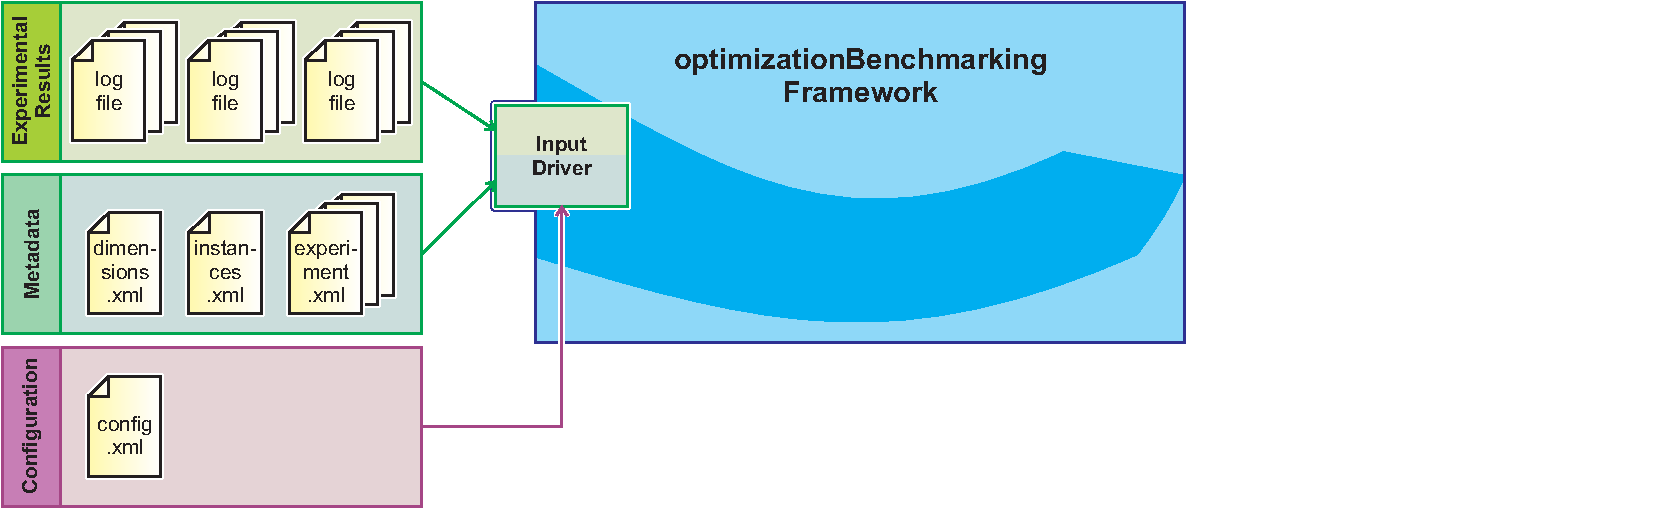
\includegraphics[width=0.9\paperwidth]{graphics/flow/flow_config_1_config}}{0.05}{0.16}%
\locate{13}{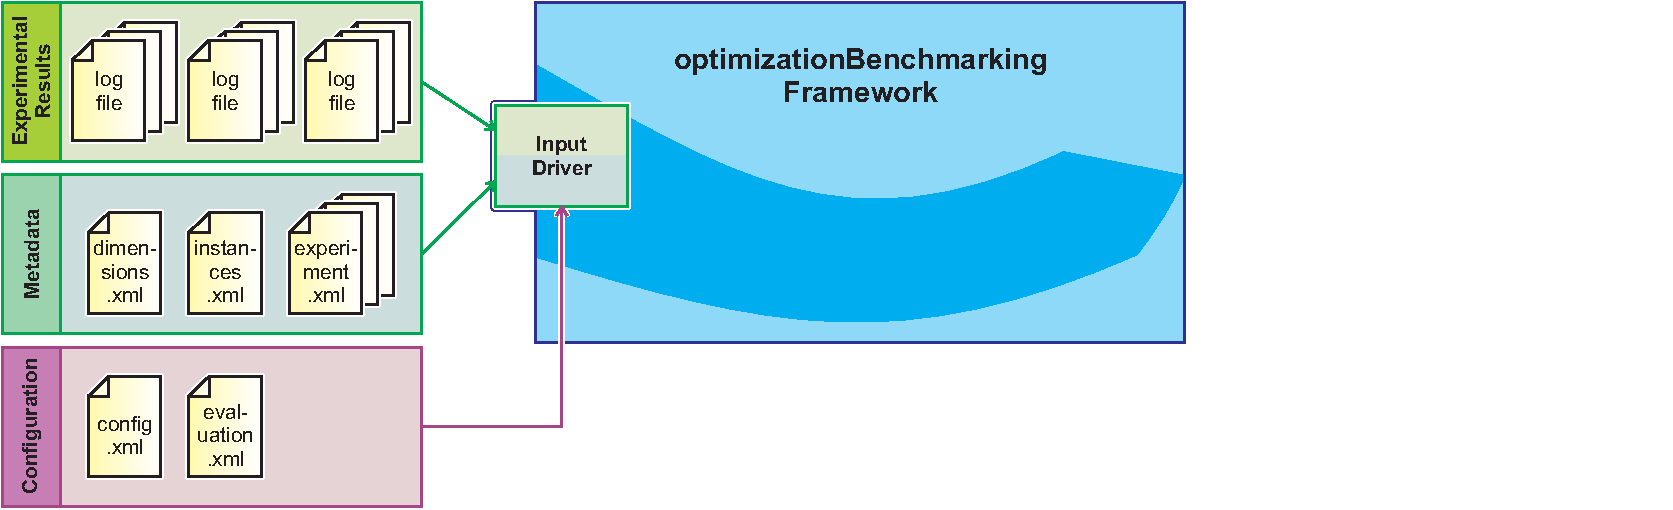
\includegraphics[width=0.9\paperwidth]{graphics/flow/flow_config_2_evaluation}}{0.05}{0.16}%
\locate{14-15}{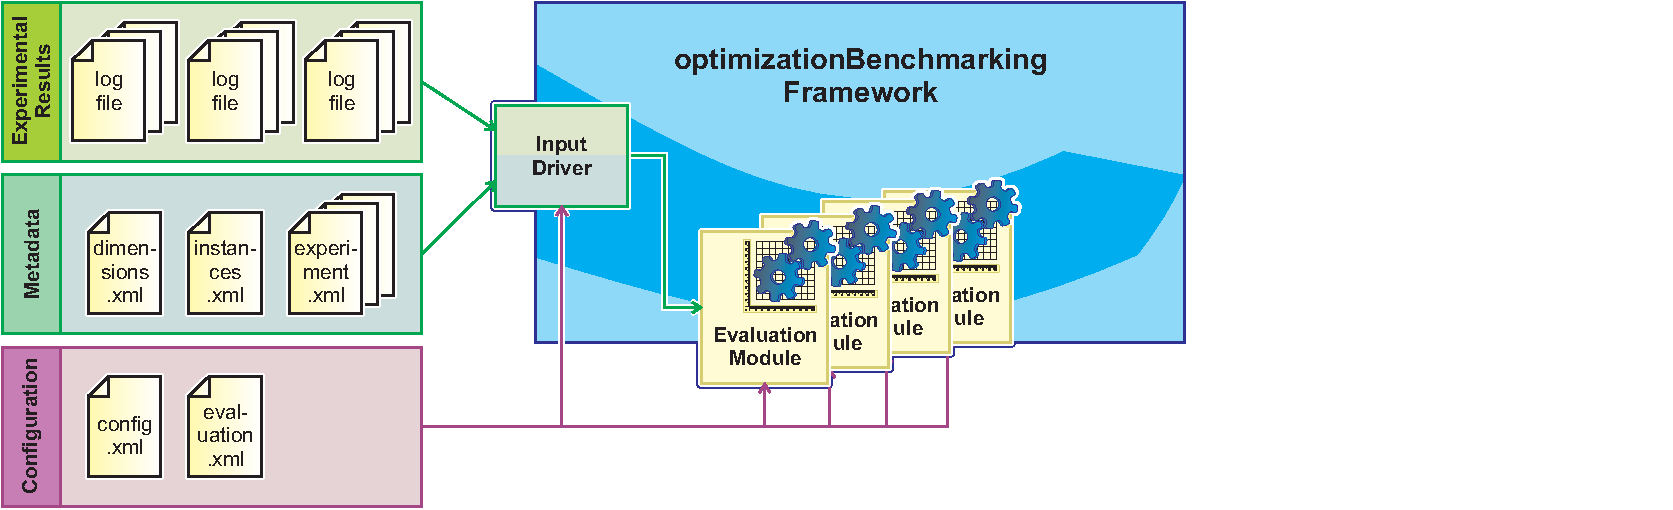
\includegraphics[width=0.9\paperwidth]{graphics/flow/flow_evaluation}}{0.05}{0.16}%
\locate{16}{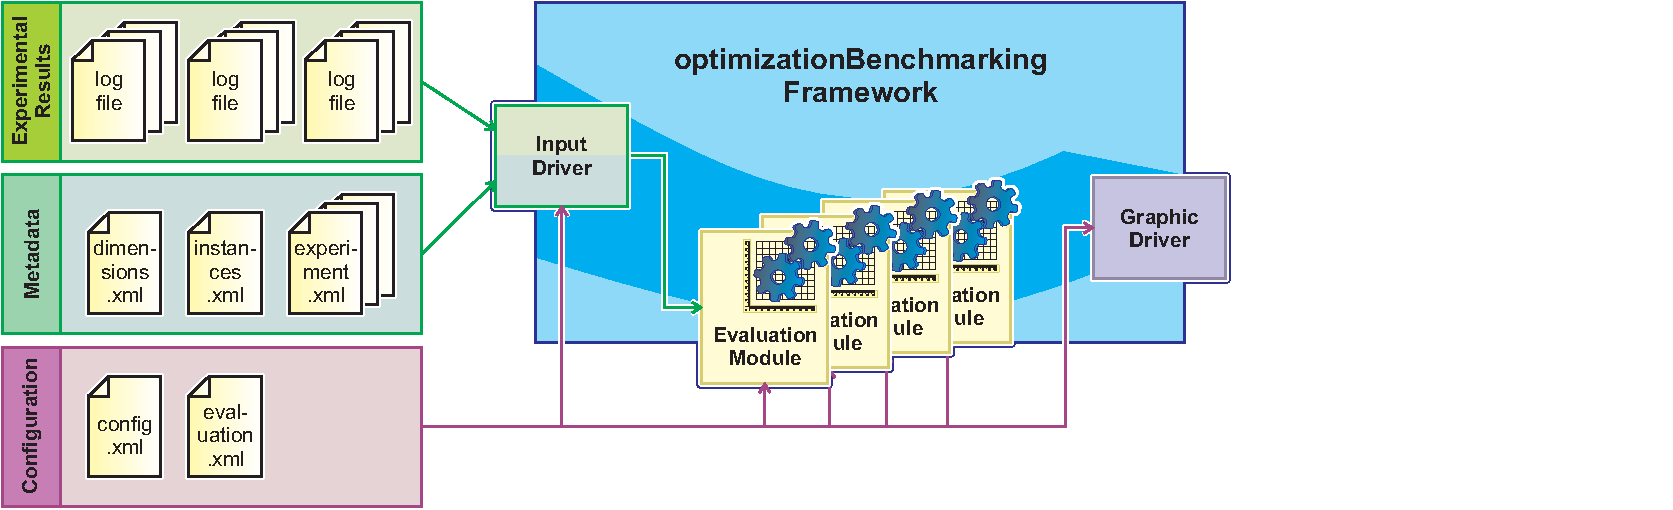
\includegraphics[width=0.9\paperwidth]{graphics/flow/flow_output_1_graphic}}{0.05}{0.16}%
\locate{17}{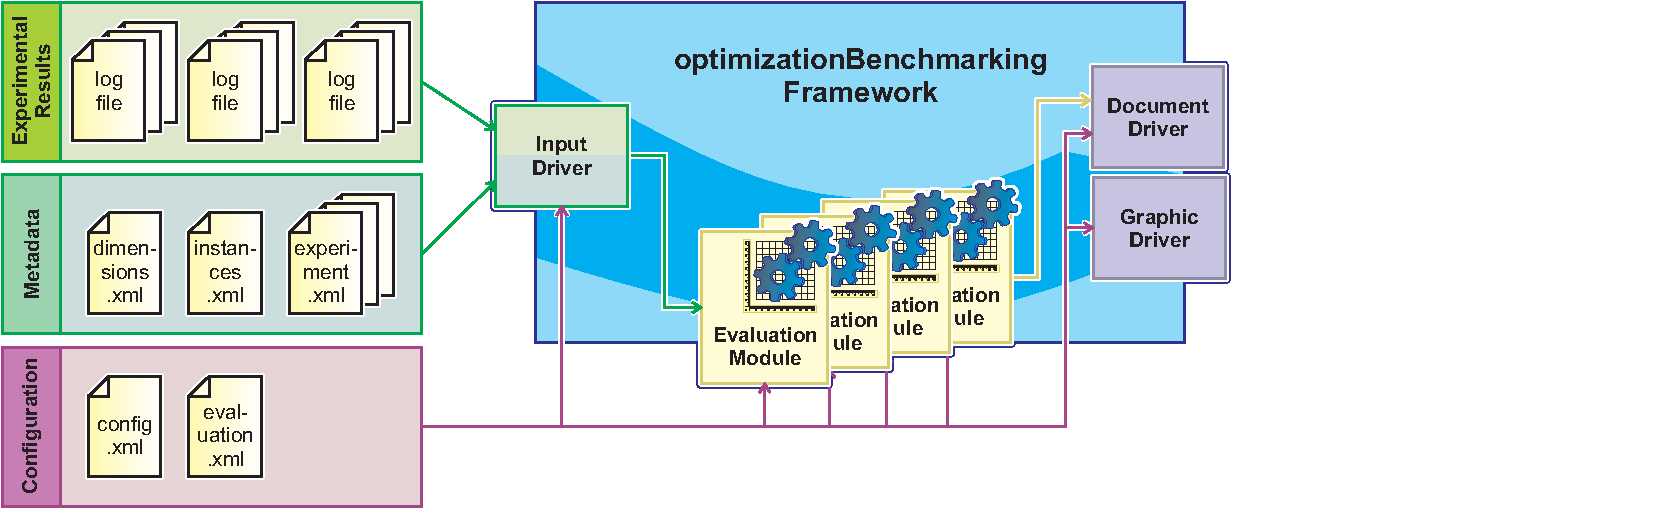
\includegraphics[width=0.9\paperwidth]{graphics/flow/flow_output_2_document}}{0.05}{0.16}%
\locate{18}{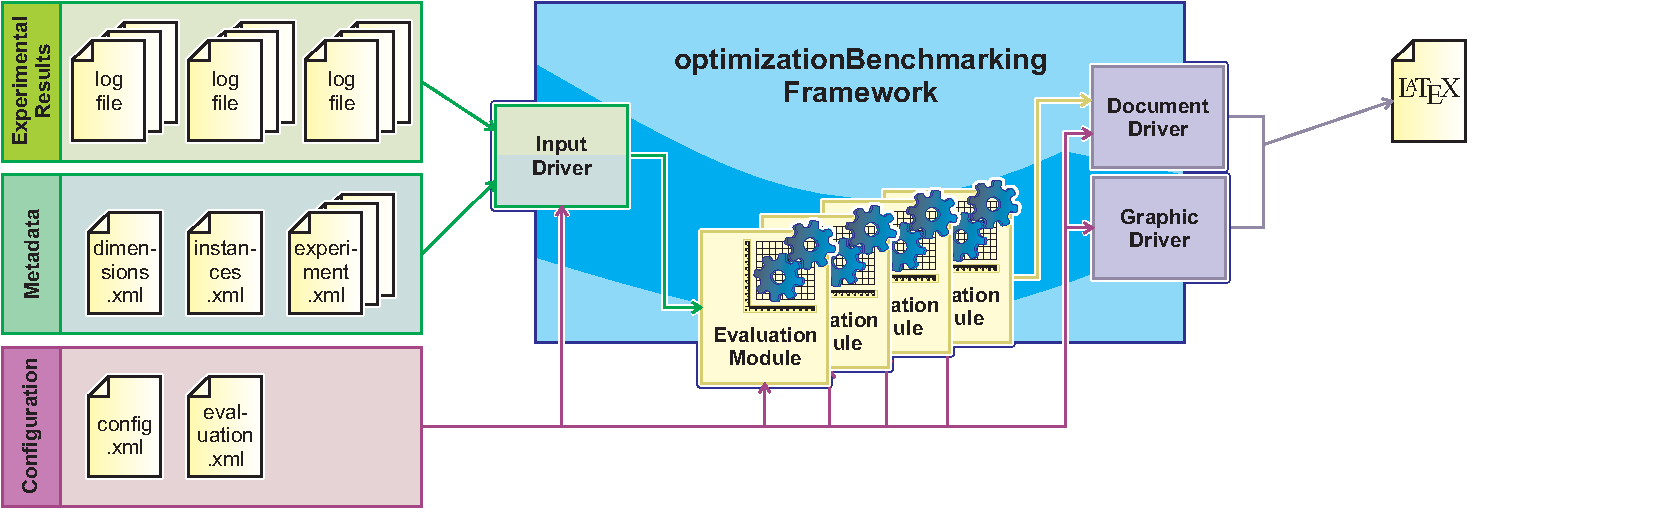
\includegraphics[width=0.9\paperwidth]{graphics/flow/flow_output_3_latex}}{0.05}{0.16}%
\locate{19-21}{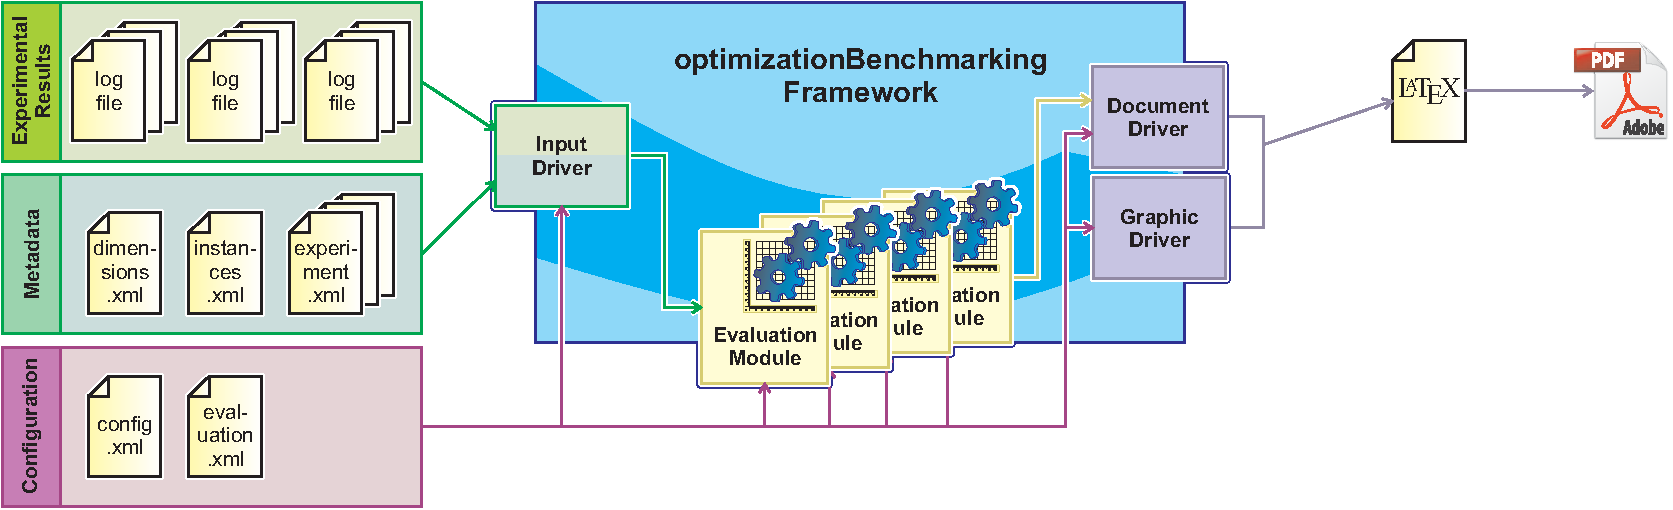
\includegraphics[width=0.9\paperwidth]{graphics/flow/flow_output_4_pdf}}{0.05}{0.16}%
\locate{22}{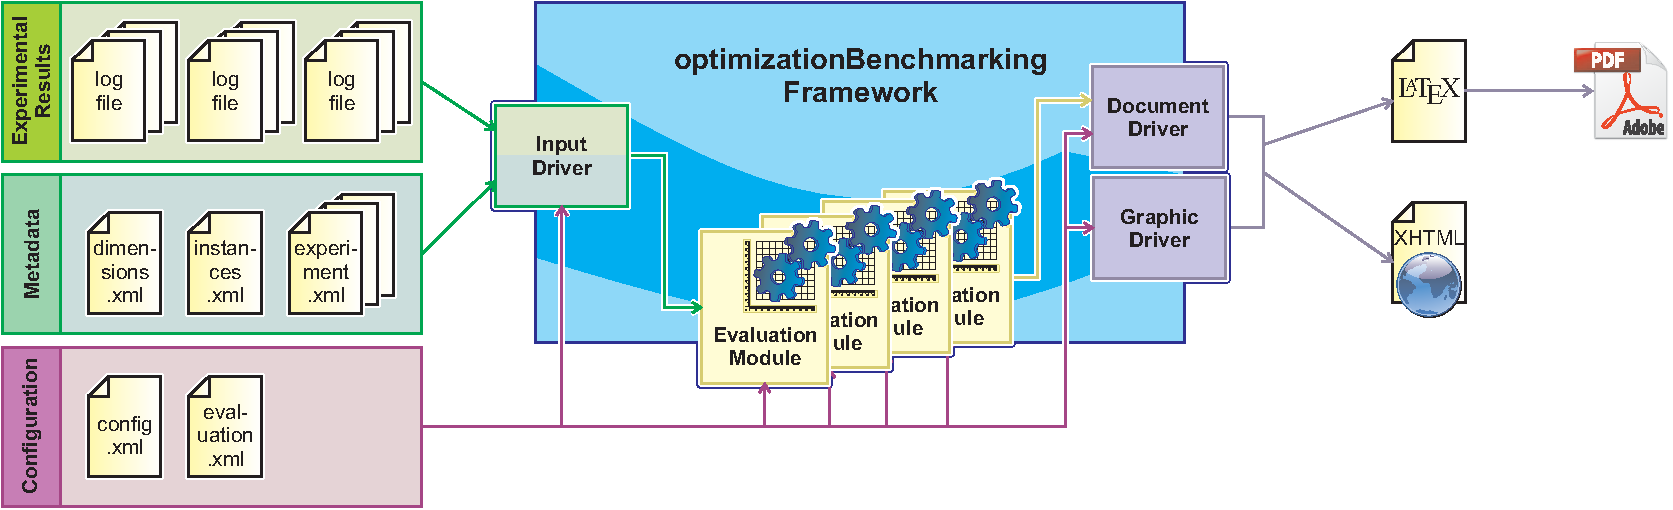
\includegraphics[width=0.9\paperwidth]{graphics/flow/flow_output_5_xhtml}}{0.05}{0.16}%
\locate{23-}{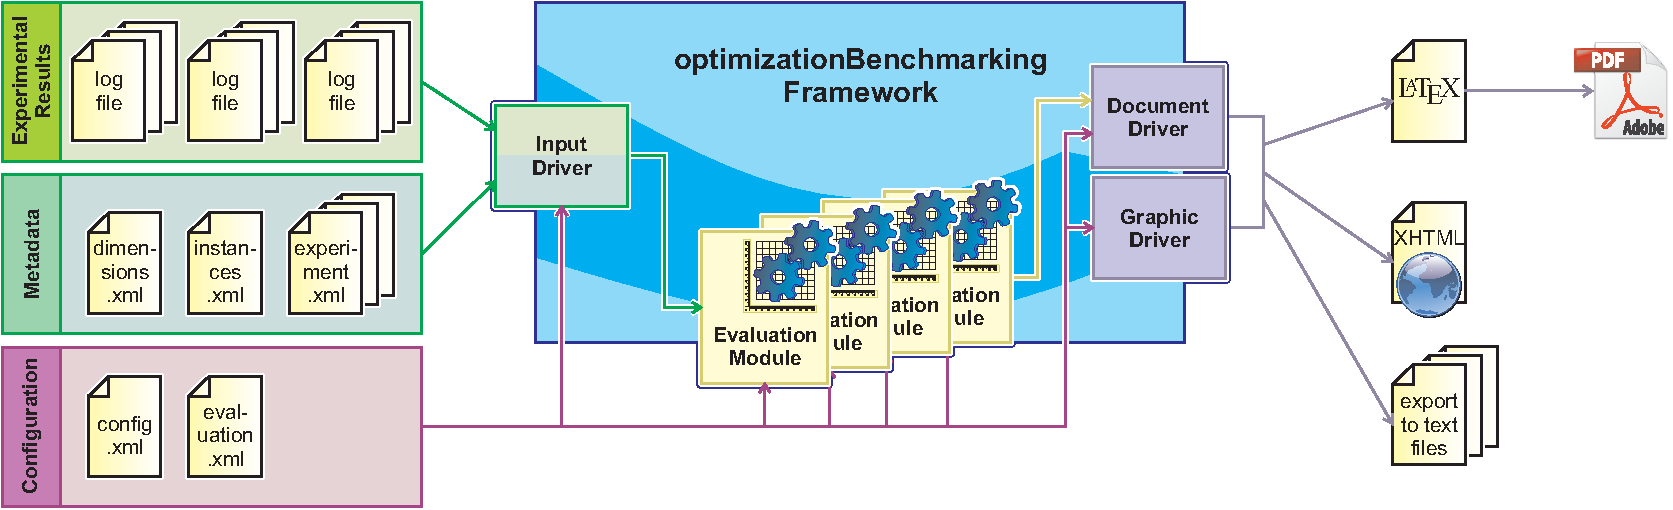
\includegraphics[width=0.9\paperwidth]{graphics/flow/flow}}{0.05}{0.16}%
%
\only<2->{%
\begin{small}%
\begin{itemize}%
%
\only<-9>{%
\item We got a couple of log files for each experiment\uncover<3->{: 6 experiments in our example, each with $10\times 10\times 20=\numprint{2000}$ log files}%
%}%
%
%\only<4-5>{%
\item<4-> We specify which dimensions we have measured\uncover<5->{: \measureFEs, \measureRuntime, and \measureObjectiveValue\ in our example\uncover<-5>{ (\alert{demo})}}%
%}%
%
%\only<6-7>{%
\item<6-> We specify which benchmark instances we have and what their features are\uncover<7->{: $10\times 10$ instances in our example, with features \maxSatVariables\ and \maxSatClauses\uncover<-7>{ (\alert{demo})}}%
%}%
%
%\only<8-9>{%
\item<8-> For each experiment, we specify the parameters\uncover<9->{: in our example, these are \texttt{algorithm}, \texttt{operator}, \texttt{restart}\uncover<-9>{ (\alert{demo})}}%
}%
%
\only<10-13>{%
\item<10-> An \inQuotes{input driver} loads the data\uncover<11->{: most commonly, the data will be in Comma-, Tab-, or Space-Separated-Values format (\textit{CSV}), but we also support \bbob\expandafter\scitep{\bbobReferences} and \tspSuite\expandafter\scitep{\tspSuiteReferences}}%
%}%
%
%\only<12>{%
\item<12-> Via a configuration file, we choose which input and output formats to use, as well as which file specifies the evaluation process%
%}%
%
%\only<13>{%
\item<13-> The \texttt{evaluation.xml} specifies \emph{how} to evaluate the data, i.e., which evaluation modules to apply%
}%
%
\only<14-15>{%
\item<14-> An evaluation module prints on particular type of information about an experiment or experiment set, such as the ECDF, or a table with final results, etc\dots%
\item<15-> Evaluation modules can be applied multiple times, with different configurations (e.g., we can plot ECDFs for different target solution qualities)%
}%
%
\only<16>{%
\item<16-> We can choose among several different formats to be used for graphics, including EPS\scitep{A1992EPFFS}, PDF\scitep{ISO320002008}, PGF (\LaTeX), SVG(Z), EMF, PNG\scitep{RFC2083}, GIF\scitep{CI1990GIFV8}, BMP, and JPG%
\\\strut%
\vspace{0.19\paperheight}%
\strut\\%
}%
%
%
\only<17-21>{%
\item<17-> We can also choose among different formats for the report documents, including\only<-17>{\dots}%
%
\uncover<18-21>{ %
\LaTeX\scitep{MGBCR2004TLC,GMS1994TLC,L1994LADPSUGARM,OPHS2011TNSSITLOLI1M}\only<21->{, XHTML\scitep{W3C2010XHTML,C2009NPOHXADHC}\only<22->{, and export to other programs}}\uncover<19-20>{:%
\begin{itemize}%
\item can automatically be compiled to PDF\scitep{ISO320002008}, if a \LaTeX\ compiler (such as TeXLive\scitep{TEXLIVE} or MiKTeX\scitep{MIKTEX}) is auto-detected%
\item<20-> different document classes, such as IEEEtran\scitep{IEEETRAN}, Springer LLNCS\scitep{SPRINGERLNCS}, ACM sig-alternate\scitep{ACMSIGALTERNATE} can be chosen%
\item<21-> graphic sizes and fonts used in graphics are automatically adapted to document class%
\end{itemize}%
}}%
}%
%
\only<22->{\only<-27>{%
\item<22-> We can also choose among different formats for the report documents, including \LaTeX\only<23->{, }\only<-22>{ and }XHTML\scitep{W3C2010XHTML}%
\only<22>{ for quick viewing in a browser}%
\only<23->{, and a plain text format to export results to other applications}}%
%
\item<24-> Evaluation Modules as well as Input, Document, and Graphic Drivers can easily be added\uncover<25->{: %
implement the corresponding interface%
\uncover<26->{%
, put your class into the classpath%
\uncover<27->{%
, and tell the system to use it in the \texttt{config.xml} or \texttt{evaluation.xml}\dots%
%
\only<28->{%
\item<28-> GUI has simple editors and help for all setup, configuration, and meta-data%
}%
%
}}}%
\only<22>{%
\strut\\\medskip\strut%
}%
\only<23->{%
\strut\medskip\strut%
}%
}%
%
\end{itemize}%
\end{small}}%
%
\end{frame}%
%
%
\begin{frame}%
\frametitle{Usage Summary}%
\begin{enumerate}%
\item Implement your optimization or Machine Learning or whatever algorithm%
\item<2-> Select a set of benchmark instances%
\item<3-> Run experiments and obtain one output folder per experiment with log files\medskip%
\item<4-> Put \texttt{dimensions.xml} into results folder (write it with the GUI)%
\item<5-> Put \texttt{instances.xml} into results folder (write it with the GUI)%
\item<6-> Put one \texttt{experiment.xml} into each experiment output folder (write it with the GUI)%
\item<7-> Define your evaluation process in a file \texttt{evaluation.xml} (write it with the GUI)%
\item<8-> Execute \optimizationBenchmarking\ evaluator%
\end{enumerate}%
\end{frame}%
%
%
%
\section{Conclusions}%
%
\begin{frame}%
\frametitle{Conclusions}%
\begin{itemize}%
\item I have presented a very first version of the evaluator GUI component of the \optimizationBenchmarking\ framework%
\item<2-> It can already load and evaluate performance data from \emph{your} optimization or Machine Learning algorithm%
\item<3-> It can help \emph{you} to understand what the strengths and weaknesses of \emph{your} algorithm are%
\item<4-> It produces figures ready for use in \emph{your} publication%
\item<5-> {\dots}and these figures are optimized (size, fonts) for the journal or conference \emph{you} want to submit to.%
\item<6-> Btw, you could even compare general algorithms (like GAs and HC) on entirely different problem types at once (like MAX-SAT and BBOB) by making the problem type an instance feature\dots%  
\end{itemize}%
%%
\end{frame}
%
%
\begin{frame}%
\frametitle{Future Work: Short-Term}%
\begin{itemize}%
\item Add more evaluation modules, to reach the power of \tspSuite\expandafter\sciptep{\tspSuiteReferences}, e.g., add automated algorithm ranking%
\item<2-> Publish overview paper about our system to publish it more widely\dots\ {\dots}when it's ready%
\item<3-> Publicize the use \optimizationBenchmarking\ to our colleagues (citations will come in\dots)%
\item<4-> Position tool as a central quality control utility for optimization and Machine Learning applications%
\item<5-> Improve features based on feedback%
\end{itemize}%
%%
\end{frame}
%
\begin{frame}%
\frametitle{Future Work: Long-Term}%
\begin{itemize}%
\item Scout for new interesting ways to evaluate optimization and Machine Learning algorithms and implement them as evaluator modules%
\item<2-> In Progress: We could use clustering to group algorithms by their behavior or problems by their hardness%
\item<3-> Btw: This is Big Data, since we can collect \emph{much} information\dots%
\end{itemize}%
\end{frame}%
%%
%
\endPresentation%
%
\appendices%
%
%
\subsection{\maxSat\ Example: Details}%
\pdfbookmark[2]{\maxSat\ Example: Details}{maxSatExampleDetails}%
%
%%
\gdef\maxSatClauses{\textcolor{red}{\ensuremath{k}}}%
\gdef\maxSatVariables{\textcolor{green}{\ensuremath{n}}}%
\gdef\maxSatVariable{\ensuremath{x}}%
\gdef\maxSatVariablei#1{\ensuremath{\maxSatVariable_{#1}}}%
\gdef\maxSatFormula{\ensuremath{B}}%
%%
\begin{frame}[label=maxSatDemoStart]%
\frametitle{\maxSat: Output and Analysis}%
\centering{\LARGE{\textbf{\alert{\maxSat: Output and Analysis}}}}%
\bigskip\begin{itemize}%
\item Here we discuss the details of the \maxSat\ example%
\item The following slides can replace the demo, if for some reason running the demo is not possible or did not work out\dots%
\item The evaluation aspects are part of this example.%
\end{itemize}%
\bigskip%
\centering\scalebox{1.8}{\hyperlink{maxSatInteractiveDemoStart}{\beamergotobutton{go back to interactive demo slides}}}%
\end{frame}%
%%
%
\begin{frame}[t]%
\frametitle{ECDF}%
\begin{itemize}%
\item We can plot the Empirical (Cumulative) Distribution Function (ECDF)\scitep{HAFR2012RPBBOBES,HS1998ELVAPAR,TH2004UAIAEEFSAFSAMS,WCTLTCMY2014BOAAOSFFTTSP} for us, which provides the fraction of runs that have found the solution for their respective problem at a given point in time.%  
\end{itemize}%
%
\locateWithCaption{2-6}{%
\strut\vbox to 0.475\paperheight{\vfil%
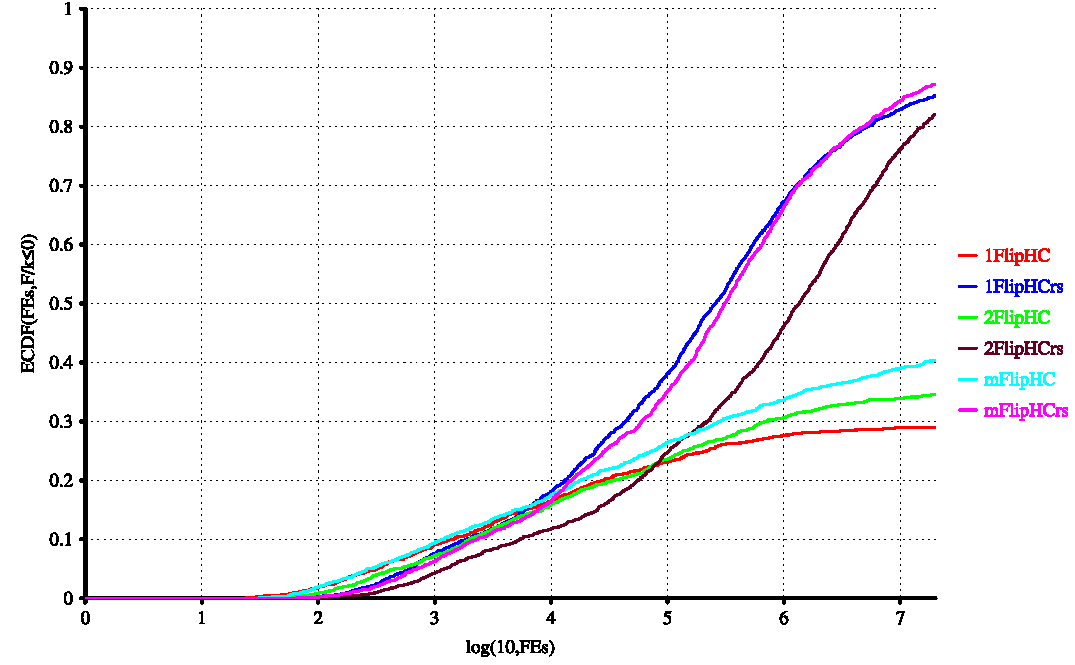
\includegraphics[scale=0.425]{graphics/maxsat_example/ECDF_log_10_FEs_F_k_0/IEEEtran_ECDF_log_10_FEs_F_k_0}%
\strut\hfill\strut%
}%
}{%
The ECDF in over all 100 benchmark instances for time measure \measureFEs\ (log-scaled\only<6->{\alert{, optimized for \texttt{IEEEtran} and two figures per row}}).%
}{0.0375}{0.34}{0.925}%%
%
\locateWithCaption{7}{%
\strut\vbox to 0.475\paperheight{\vfil%
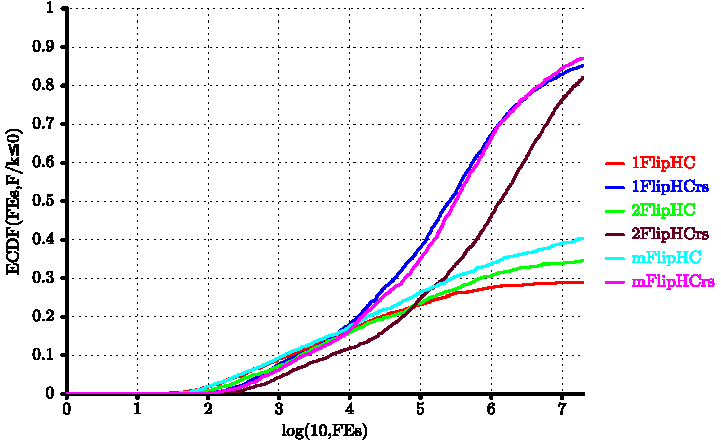
\includegraphics[scale=0.425]{graphics/maxsat_example/ECDF_log_10_FEs_F_k_0/LNCS_ECDF_log_10_FEs_F_k_0}%
\strut\hfill\strut}%
}{%
The ECDF in over all 100 benchmark instances (log-scaled, \alert{optimized for \texttt{LNCS} and two figures per row}).%
}{0.0375}{0.34}{0.925}%
%
\locateWithCaption{8}{%
\strut\vbox to 0.475\paperheight{\vfil%
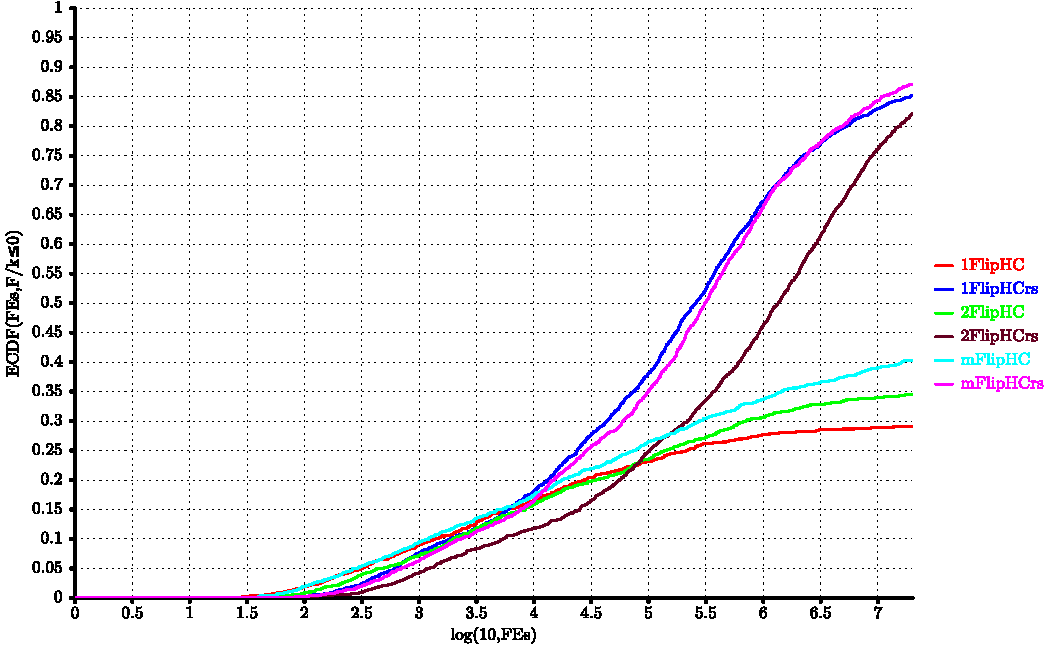
\includegraphics[scale=0.425]{graphics/maxsat_example/ECDF_log_10_FEs_F_k_0/SigAlternate_ECDF_log_10_FEs_F_k_0}%
\strut\hfill\strut}%
}{%
The ECDF in over all 100 benchmark instances (log-scaled, \alert{optimized for \texttt{sig-alternate} and two figures per row}).%
}{0.0375}{0.34}{0.925}%
%
\locateWithCaption{9}{%
\strut\vbox to 0.475\paperheight{\vfil%
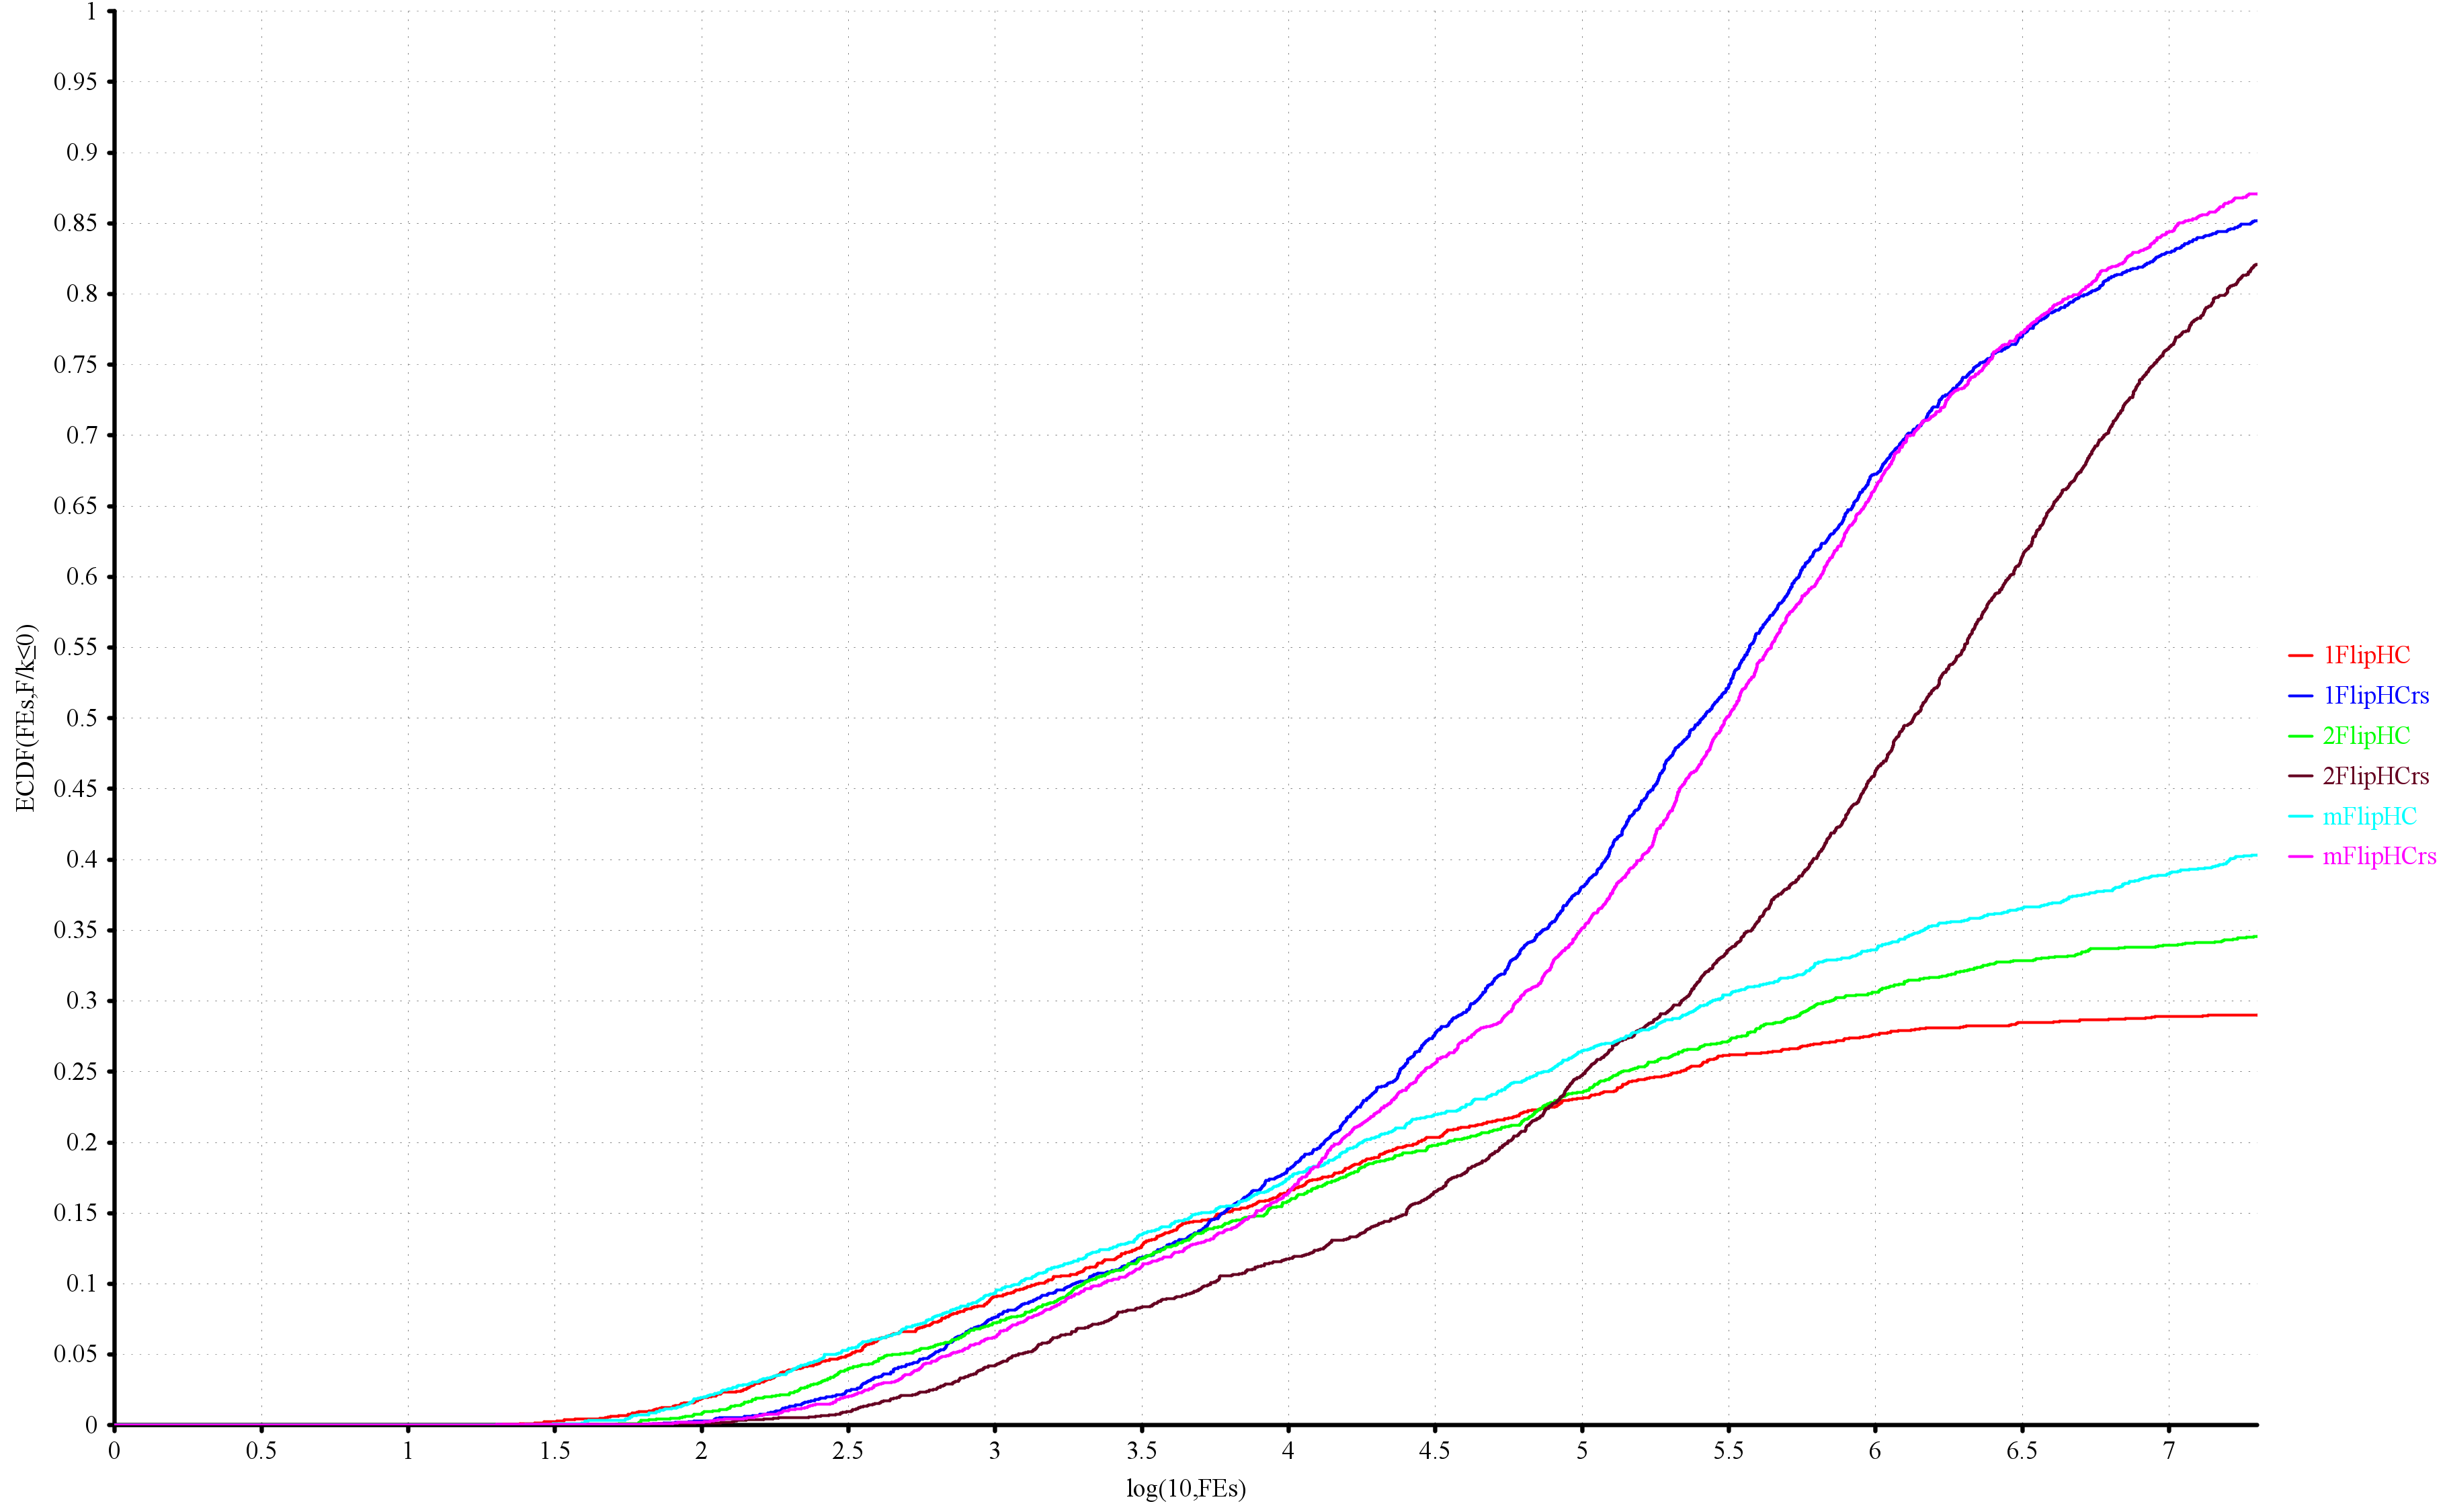
\includegraphics[width=0.6\paperwidth]{graphics/maxsat_example/ECDF_log_10_FEs_F_k_0/XHTML_ECDF_log_10_FEs_F_k_0}%
\strut\hfill\strut}%
}{%
The ECDF in over all 100 benchmark instances (log-scaled, \alert{optimized for \texttt{XHTML} and two figures per row}).%
}{0.0375}{0.34}{0.925}%
%
\locate{3-}{\parbox{0.35\paperwidth}{\small%
\begin{itemize}%
\item the methods with restarts solve more problems (up to 90\%!)%
\item<4-> plain $m$-flips are better than 2-flips are better than 1-flips%
\item<5-> oddly, for restart HCers, there is a tie between the $m$- and 1-flip versions 
\end{itemize}%
}}{0.625}{0.3}%
%
\end{frame}%
%
\begin{frame}%
\frametitle{ECDF for Different Values of \scalebox{1.3}{\ensuremath{\mathbf{\maxSatVariables}}}}%
%
\locate{1-}{%
\parbox{0.234\paperwidth}{\raggedright\small{%
\only<-1>{We now look at the ECDF for different values of \maxSatVariables\ and a goal of 1\% unsatisfied clauses over \measureRuntime\ (log-scaled).}%
\only<2>{For $\maxSatVariables=20$, the methods with restarts are better.}%
\only<3>{But for $\maxSatVariables\geq 50$, those without reach the goal faster.}%
\only<4>{It seems that 1\% unsatisfied clauses can be reached with 1-flips and without restarts.}%
\only<5>{The 2-flip operator again performs worst.}%
\only<6>{It looks as if it gets easier to attain a 1\% error margin if \maxSatVariables\ increases (all ECDFs reach 1).}%
\only<7-8>{For small problems, 1-flip is slightly faster than $m$-flip.}%
\only<9>{For larger problems, $m$-flip becomes slightly faster.}%
\only<10>{All in all, similar behavior over all scales (reaching 1\% error seems to be easy).}%
\only<11->{Only required runtime increases by up to 100 times.}%
}}}{0.013}{0.187}%
%
\locate{1-}{%
\parbox{0.234375\paperwidth}{\centering%
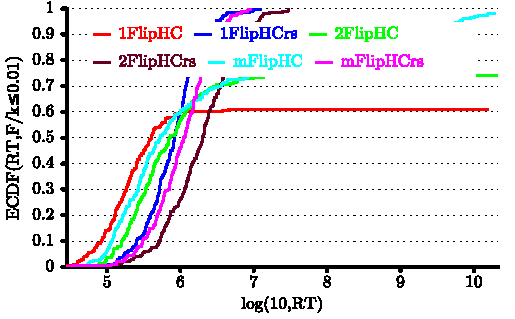
\includegraphics[width=0.234375\paperwidth]{graphics/maxsat_example/ECDF_log_10_RT_F_k_0_01_distinct_n/SigAlternate_ECDF_log_10_RT_F_k_0_01_distinct_n_legend}%
\\\scriptsize{legend}}%
}{0.259375}{0.18}%
%
\locate{2-}{%
\parbox{0.234375\paperwidth}{\centering%
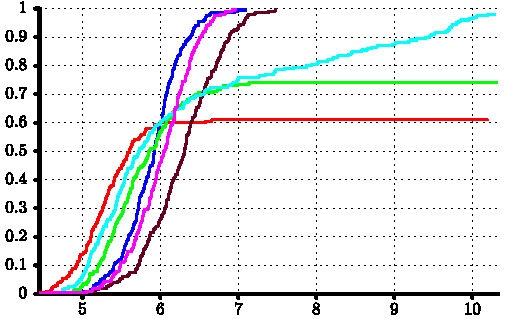
\includegraphics[width=0.234375\paperwidth]{graphics/maxsat_example/ECDF_log_10_RT_F_k_0_01_distinct_n/SigAlternate_ECDF_log_10_RT_F_k_0_01_distinct_n_20}%
\\\scriptsize{$\maxSatVariables=20$}}%
}{0.50625}{0.18}%
%
\locate{3-}{%
\parbox{0.234375\paperwidth}{\centering%
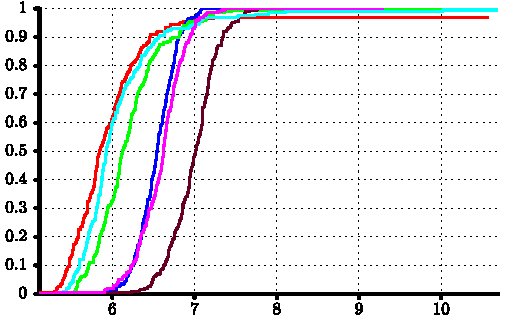
\includegraphics[width=0.234375\paperwidth]{graphics/maxsat_example/ECDF_log_10_RT_F_k_0_01_distinct_n/SigAlternate_ECDF_log_10_RT_F_k_0_01_distinct_n_50}%
\\\scriptsize{$\maxSatVariables=50$}}%
}{0.753125}{0.18}%
%
\locate{4-}{%
\parbox{0.234375\paperwidth}{\centering%
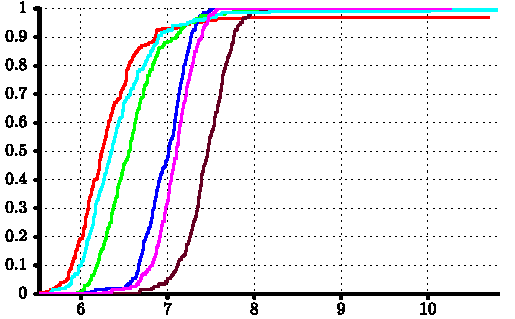
\includegraphics[width=0.234375\paperwidth]{graphics/maxsat_example/ECDF_log_10_RT_F_k_0_01_distinct_n/SigAlternate_ECDF_log_10_RT_F_k_0_01_distinct_n_75}%
\\\scriptsize{$\maxSatVariables=75$}}%
}{0.0125}{0.443333333333333}%
%
\locate{5-}{%
\parbox{0.234375\paperwidth}{\centering%
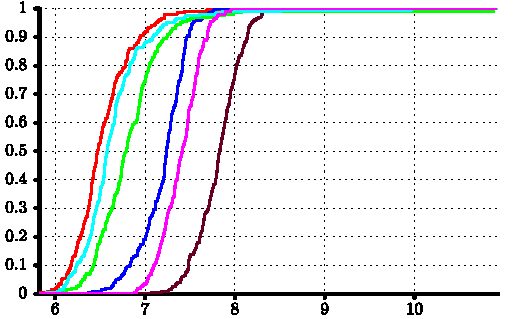
\includegraphics[width=0.234375\paperwidth]{graphics/maxsat_example/ECDF_log_10_RT_F_k_0_01_distinct_n/SigAlternate_ECDF_log_10_RT_F_k_0_01_distinct_n_100}%
\\\scriptsize{$\maxSatVariables=100$}}%
}{0.259375}{0.443333333333333}%
%
\locate{6-}{%
\parbox{0.234375\paperwidth}{\centering%
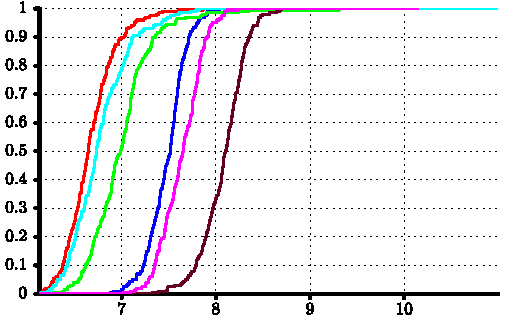
\includegraphics[width=0.234375\paperwidth]{graphics/maxsat_example/ECDF_log_10_RT_F_k_0_01_distinct_n/SigAlternate_ECDF_log_10_RT_F_k_0_01_distinct_n_125}%
\\\scriptsize{$\maxSatVariables=125$}}%
}{0.50625}{0.443333333333333}%
%
\locate{7-}{%
\parbox{0.234375\paperwidth}{\centering%
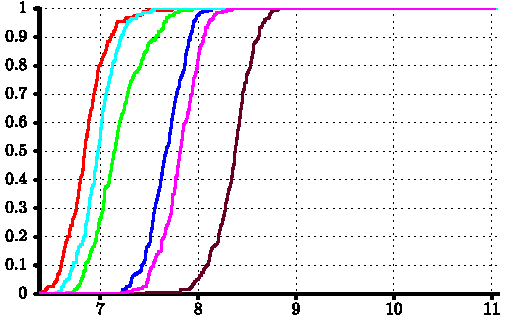
\includegraphics[width=0.234375\paperwidth]{graphics/maxsat_example/ECDF_log_10_RT_F_k_0_01_distinct_n/SigAlternate_ECDF_log_10_RT_F_k_0_01_distinct_n_150}%
\\\scriptsize{$\maxSatVariables=150$}}%
}{0.753125}{0.443333333333333}%
%
\locate{8-}{%
\parbox{0.234375\paperwidth}{\centering%
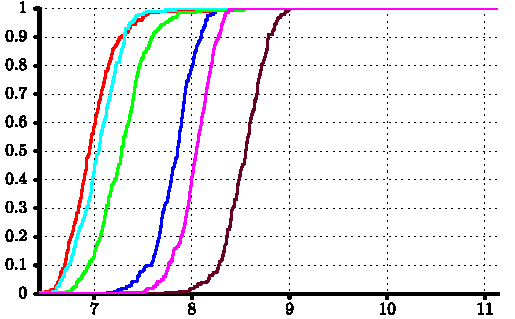
\includegraphics[width=0.234375\paperwidth]{graphics/maxsat_example/ECDF_log_10_RT_F_k_0_01_distinct_n/SigAlternate_ECDF_log_10_RT_F_k_0_01_distinct_n_175}%
\\\scriptsize{$\maxSatVariables=175$}}%
}{0.0125}{0.706666666666667}%
%
\locate{9-}{%
\parbox{0.234375\paperwidth}{\centering%
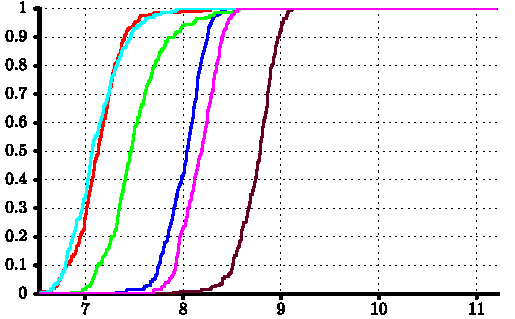
\includegraphics[width=0.234375\paperwidth]{graphics/maxsat_example/ECDF_log_10_RT_F_k_0_01_distinct_n/SigAlternate_ECDF_log_10_RT_F_k_0_01_distinct_n_200}%
\\\scriptsize{$\maxSatVariables=200$}}%
}{0.259375}{0.706666666666667}%%
%
\locate{10-}{%
\parbox{0.234375\paperwidth}{\centering%
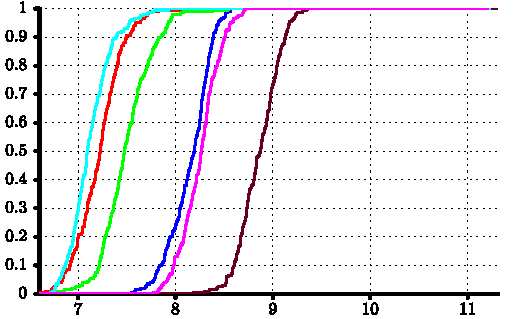
\includegraphics[width=0.234375\paperwidth]{graphics/maxsat_example/ECDF_log_10_RT_F_k_0_01_distinct_n/SigAlternate_ECDF_log_10_RT_F_k_0_01_distinct_n_225}%
\\\scriptsize{$\maxSatVariables=225$}}%
}{0.50625}{0.706666666666667}%
%
\locate{11-}{%
\parbox{0.234375\paperwidth}{\centering%
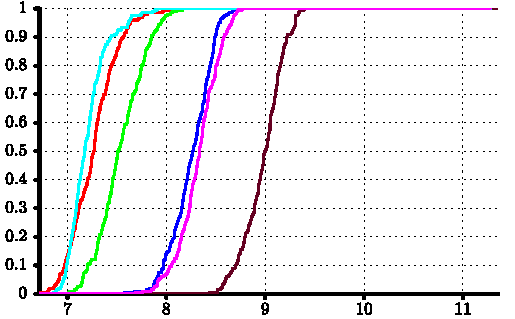
\includegraphics[width=0.234375\paperwidth]{graphics/maxsat_example/ECDF_log_10_RT_F_k_0_01_distinct_n/SigAlternate_ECDF_log_10_RT_F_k_0_01_distinct_n_250}%
\\\scriptsize{$\maxSatVariables=250$}}%
}{0.753125}{0.706666666666667}%
%
\end{frame}%
%
%
\begin{frame}%
\frametitle{Progress for Different Values of \scalebox{1.3}{\ensuremath{\mathbf{\maxSatClauses}}}}%
%
\locate{1-}{%
\parbox{0.234\paperwidth}{\raggedright\small{%
\only<-1>{We now look at the progress curves (\measureObjectiveValue\ over \measureFEs\ divided by\footnote<1>{We normalize \measureFEs\ with \maxSatVariables\ in the hope to make the time measure comparable over different \maxSatVariables.} \maxSatVariables, log-scaled) for different values of \maxSatClauses.}%
\only<2>{For very small-scale problems, all algorithms behave similar.}%
\only<3>{But soon, two groups form: with and without restarts.}%
\only<4>{Algorithms using \emph{my example restart policy} seem to be slower.}%
\only<5>{The gap increases with rising \maxSatClauses}%
\only<6>{Thus, we find: algorithms with my restart policy are slower than those without\dots}%
\only<7>{{\dots}but from the ECDF we know they can solve more problems eventually.}%
\only<8>{For all scales, the initial random solutions, seem to have about 12\% of unsatisfied clauses (in median).}%
\only<9->{Convergence seems to happen between 100\maxSatVariables\ and 1000\maxSatVariables}%
}}}{0.013}{0.187}%
%
\locate{1-}{%
\parbox{0.234375\paperwidth}{\centering%
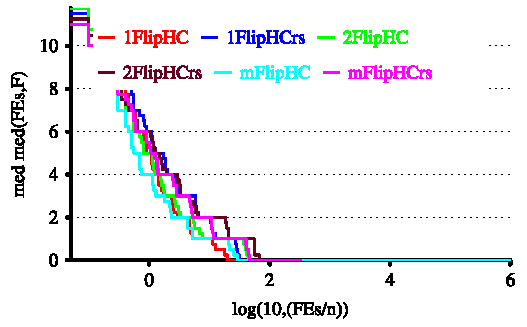
\includegraphics[width=0.234375\paperwidth]{graphics/maxsat_example/med_med_log_10_FEs_n_F_distinct_k/IEEEtran_med_med_log_10_FEs_n_F_distinct_k_legend}%
\\\scriptsize{legend}}%
}{0.259375}{0.18}%
%
\locate{2-}{%
\parbox{0.234375\paperwidth}{\centering%
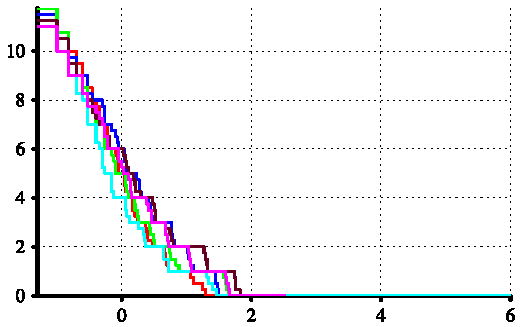
\includegraphics[width=0.234375\paperwidth]{graphics/maxsat_example/med_med_log_10_FEs_n_F_distinct_k/IEEEtran_med_med_log_10_FEs_n_F_distinct_k_91}%
\\\scriptsize{$\maxSatClauses=91$}}%
}{0.50625}{0.18}%
%
\locate{3-}{%
\parbox{0.234375\paperwidth}{\centering%
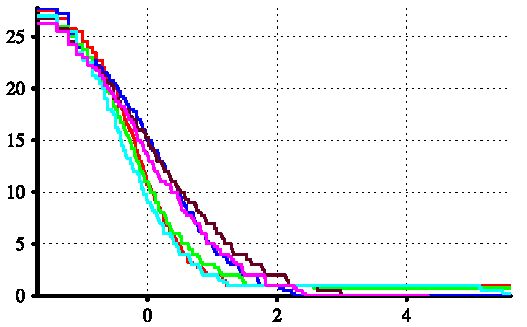
\includegraphics[width=0.234375\paperwidth]{graphics/maxsat_example/med_med_log_10_FEs_n_F_distinct_k/IEEEtran_med_med_log_10_FEs_n_F_distinct_k_218}%
\\\scriptsize{$\maxSatClauses=218$}}%
}{0.753125}{0.18}%
%
\locate{4-}{%
\parbox{0.234375\paperwidth}{\centering%
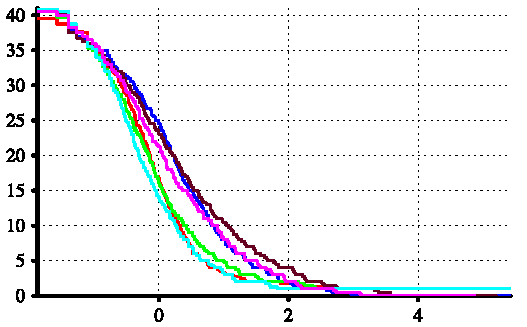
\includegraphics[width=0.234375\paperwidth]{graphics/maxsat_example/med_med_log_10_FEs_n_F_distinct_k/IEEEtran_med_med_log_10_FEs_n_F_distinct_k_325}%
\\\scriptsize{$\maxSatClauses=325$}}%
}{0.0125}{0.443333333333333}%
%
\locate{5-}{%
\parbox{0.234375\paperwidth}{\centering%
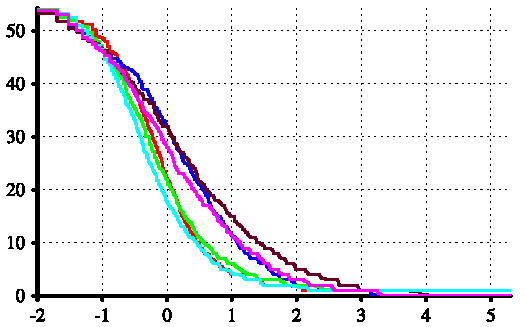
\includegraphics[width=0.234375\paperwidth]{graphics/maxsat_example/med_med_log_10_FEs_n_F_distinct_k/IEEEtran_med_med_log_10_FEs_n_F_distinct_k_430}%
\\\scriptsize{$\maxSatClauses=430$}}%
}{0.259375}{0.443333333333333}%
%
\locate{6-}{%
\parbox{0.234375\paperwidth}{\centering%
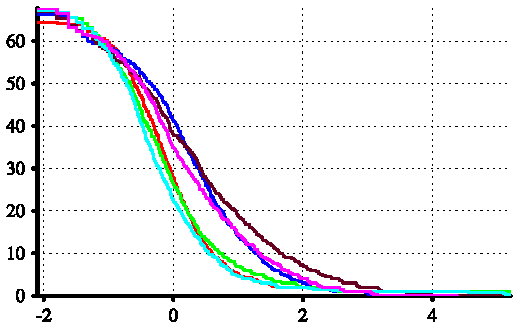
\includegraphics[width=0.234375\paperwidth]{graphics/maxsat_example/med_med_log_10_FEs_n_F_distinct_k/IEEEtran_med_med_log_10_FEs_n_F_distinct_k_538}%
\\\scriptsize{$\maxSatClauses=538$}}%
}{0.50625}{0.443333333333333}%
%
\locate{7-}{%
\parbox{0.234375\paperwidth}{\centering%
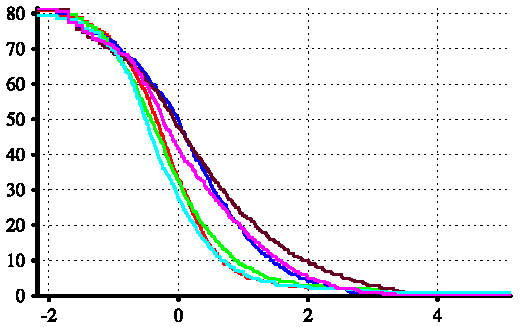
\includegraphics[width=0.234375\paperwidth]{graphics/maxsat_example/med_med_log_10_FEs_n_F_distinct_k/IEEEtran_med_med_log_10_FEs_n_F_distinct_k_645}%
\\\scriptsize{$\maxSatClauses=645$}}%
}{0.753125}{0.443333333333333}%
%
\locate{8-}{%
\parbox{0.234375\paperwidth}{\centering%
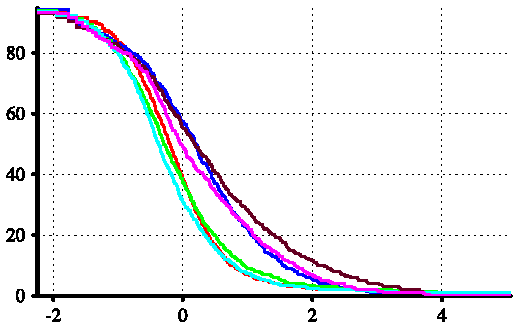
\includegraphics[width=0.234375\paperwidth]{graphics/maxsat_example/med_med_log_10_FEs_n_F_distinct_k/IEEEtran_med_med_log_10_FEs_n_F_distinct_k_753}%
\\\scriptsize{$\maxSatClauses=753$}}%
}{0.0125}{0.706666666666667}%
%
\locate{9-}{%
\parbox{0.234375\paperwidth}{\centering%
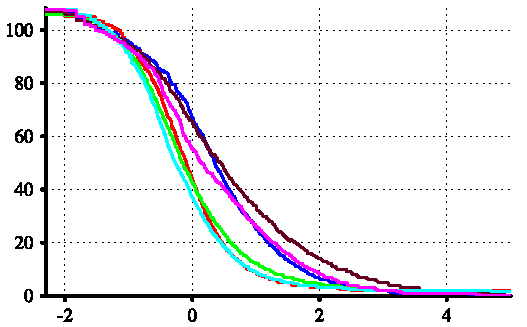
\includegraphics[width=0.234375\paperwidth]{graphics/maxsat_example/med_med_log_10_FEs_n_F_distinct_k/IEEEtran_med_med_log_10_FEs_n_F_distinct_k_860}%
\\\scriptsize{$\maxSatClauses=860$}}%
}{0.259375}{0.706666666666667}%%
%
\locate{10-}{%
\parbox{0.234375\paperwidth}{\centering%
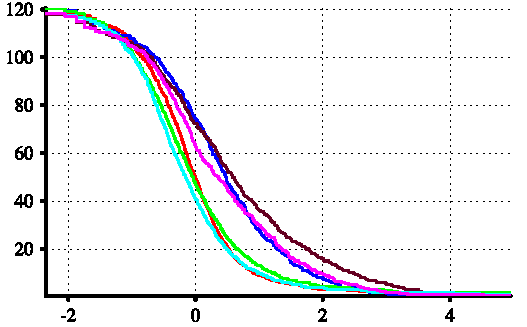
\includegraphics[width=0.234375\paperwidth]{graphics/maxsat_example/med_med_log_10_FEs_n_F_distinct_k/IEEEtran_med_med_log_10_FEs_n_F_distinct_k_960}%
\\\scriptsize{$\maxSatClauses=960$}}%
}{0.50625}{0.706666666666667}%
%
\locate{11-}{%
\parbox{0.234375\paperwidth}{\centering%
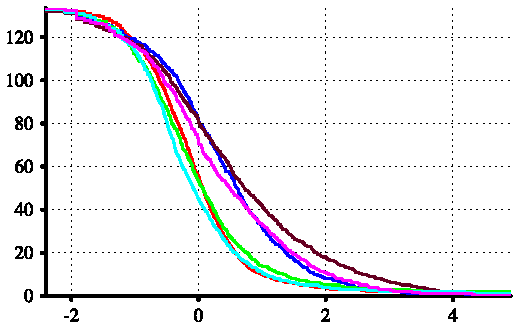
\includegraphics[width=0.234375\paperwidth]{graphics/maxsat_example/med_med_log_10_FEs_n_F_distinct_k/IEEEtran_med_med_log_10_FEs_n_F_distinct_k_1065}%
\\\scriptsize{$\maxSatClauses=1065$}}%
}{0.753125}{0.706666666666667}%
%
\end{frame}%
%
%
\begin{frame}%
\frametitle{StdDev of \measureObjectiveValue\ for Different Values of \scalebox{1.3}{\ensuremath{\mathbf{\maxSatVariables}}}}%
%
\locate{1-}{%
\parbox{0.234\paperwidth}{\raggedright\small{%
\only<-1>{Let's look at the standard deviation of the best objective value \measureObjectiveValue\ (divided by\footnote<1>{Since \measureObjectiveValue\ is always in $1\dots\maxSatClauses$, dividing it by \maxSatClauses\ normalizes it into $[0,1]$ and makes the values comparable for different \maxSatClauses\ or \maxSatVariables.} \maxSatClauses) found over \measureRuntime\ (log-scaled) for different values of \maxSatVariables.}%
\only<2>{For small-scale problems, the standard deviation seems to decrease steadily.}%
\only<3>{The reason is probably that the algorithms converge nicely.}%
\only<4>{For the methods with restarts, it reaches very close to 0.}%
\only<5>{For those without, it remains constant above 0 after some time.}%
\only<6>{These algorithms probably get stuck at different local optima in different runs.}%
\only<7>{For increasing scales, the standard deviation goes first down, then up, then farther down.}%
\only<8>{Maybe there is some kind of hard-to-attain improvement that some runs find earlier than others.}%
\only<9>{The time of convergence seems to increase for the methods with restarts with \maxSatVariables.}%
\only<10->{The early standard deviations are usually below 0.03 and highest for small \maxSatVariables.}% 
}}}{0.013}{0.187}%
%
\locate{1-}{%
\parbox{0.234375\paperwidth}{\centering%
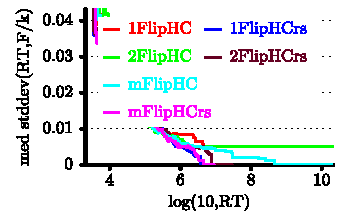
\includegraphics[width=0.234375\paperwidth]{graphics/maxsat_example/med_stddev_log_10_RT_F_k_distinct_n/LNCS_med_stddev_log_10_RT_F_k_distinct_n_legend}%
\\\scriptsize{legend}}%
}{0.259375}{0.18}%
%
\locate{2-}{%
\parbox{0.234375\paperwidth}{\centering%
\includegraphics[width=0.234375\paperwidth]{graphics/maxsat_example/med_stddev_log_10_RT_F_k_distinct_n/LNCS_med_stddev_log_10_RT_F_k_distinct_n_20}%
\\\scriptsize{$\maxSatVariables=20$}}%
}{0.50625}{0.18}%
%
\locate{3-}{%
\parbox{0.234375\paperwidth}{\centering%
\includegraphics[width=0.234375\paperwidth]{graphics/maxsat_example/med_stddev_log_10_RT_F_k_distinct_n/LNCS_med_stddev_log_10_RT_F_k_distinct_n_50}%
\\\scriptsize{$\maxSatVariables=50$}}%
}{0.753125}{0.18}%
%
\locate{4-}{%
\parbox{0.234375\paperwidth}{\centering%
\includegraphics[width=0.234375\paperwidth]{graphics/maxsat_example/med_stddev_log_10_RT_F_k_distinct_n/LNCS_med_stddev_log_10_RT_F_k_distinct_n_75}%
\\\scriptsize{$\maxSatVariables=75$}}%
}{0.0125}{0.443333333333333}%
%
\locate{5-}{%
\parbox{0.234375\paperwidth}{\centering%
\includegraphics[width=0.234375\paperwidth]{graphics/maxsat_example/med_stddev_log_10_RT_F_k_distinct_n/LNCS_med_stddev_log_10_RT_F_k_distinct_n_100}%
\\\scriptsize{$\maxSatVariables=100$}}%
}{0.259375}{0.443333333333333}%
%
\locate{6-}{%
\parbox{0.234375\paperwidth}{\centering%
\includegraphics[width=0.234375\paperwidth]{graphics/maxsat_example/med_stddev_log_10_RT_F_k_distinct_n/LNCS_med_stddev_log_10_RT_F_k_distinct_n_125}%
\\\scriptsize{$\maxSatVariables=125$}}%
}{0.50625}{0.443333333333333}%
%
\locate{7-}{%
\parbox{0.234375\paperwidth}{\centering%
\includegraphics[width=0.234375\paperwidth]{graphics/maxsat_example/med_stddev_log_10_RT_F_k_distinct_n/LNCS_med_stddev_log_10_RT_F_k_distinct_n_150}%
\\\scriptsize{$\maxSatVariables=150$}}%
}{0.753125}{0.443333333333333}%
%
\locate{8-}{%
\parbox{0.234375\paperwidth}{\centering%
\includegraphics[width=0.234375\paperwidth]{graphics/maxsat_example/med_stddev_log_10_RT_F_k_distinct_n/LNCS_med_stddev_log_10_RT_F_k_distinct_n_175}%
\\\scriptsize{$\maxSatVariables=175$}}%
}{0.0125}{0.706666666666667}%
%
\locate{9-}{%
\parbox{0.234375\paperwidth}{\centering%
\includegraphics[width=0.234375\paperwidth]{graphics/maxsat_example/med_stddev_log_10_RT_F_k_distinct_n/LNCS_med_stddev_log_10_RT_F_k_distinct_n_200}%
\\\scriptsize{$\maxSatVariables=200$}}%
}{0.259375}{0.706666666666667}%%
%
\locate{10-}{%
\parbox{0.234375\paperwidth}{\centering%
\includegraphics[width=0.234375\paperwidth]{graphics/maxsat_example/med_stddev_log_10_RT_F_k_distinct_n/LNCS_med_stddev_log_10_RT_F_k_distinct_n_225}%
\\\scriptsize{$\maxSatVariables=225$}}%
}{0.50625}{0.706666666666667}%
%
\locate{11-}{%
\parbox{0.234375\paperwidth}{\centering%
\includegraphics[width=0.234375\paperwidth]{graphics/maxsat_example/med_stddev_log_10_RT_F_k_distinct_n/LNCS_med_stddev_log_10_RT_F_k_distinct_n_250}%
\\\scriptsize{$\maxSatVariables=250$}}%
}{0.753125}{0.706666666666667}%
%
\end{frame}%
%
%%
%
\begin{frame}[t]%
\frametitle{Result}%
\only<-5>{%
\begin{itemize}%
\item The Evaluator will now produce report documents containing the requested information (and figures)%
\end{itemize}%
}%
\locate{6}{%
\parbox{\paperwidth}{%
\centering\scalebox{1.8}{\hyperlink{maxSatInteractiveDemoEnd}{\beamergotobutton{continue after end of interactive demo slides}}}%
}%
}{0}{0.16}%
%
\locateWithCaption{2-}{%
\strut\vbox to 0.475\paperheight{\vfil\fbox{%
\includegraphics[width=0.215\paperwidth,page=1]{graphics/maxsat_example/maxsat_example_reports/IEEEtran_report.pdf}%
}\strut\hfill\strut}%
}{%
first page of the report in \LaTeX\ for \texttt{IEEEtran}%
}{0.02}{0.255}{0.225}%
%
%
\locateWithCaption{3-}{%
\strut\vbox to 0.475\paperheight{\vfil\fbox{%
\includegraphics[width=0.215\paperwidth,page=1]{graphics/maxsat_example/maxsat_example_reports/LNCS_report.pdf}%
}\strut\hfill\strut}%
}{%
first page of the report in \LaTeX\ for \texttt{LNCS}%
}{0.265}{0.255}{0.225}%
%
\locateWithCaption{4-}{%
\strut\vbox to 0.475\paperheight{\vfil\fbox{%
\includegraphics[width=0.215\paperwidth,page=1]{graphics/maxsat_example/maxsat_example_reports/SigAlternate_report.pdf}%
}\strut\hfill\strut}%
}{%
first page of the report in \LaTeX\ for \texttt{sig-alternate}%
}{0.51}{0.255}{0.225}%
%
\locateWithCaption{5-}{%
\strut\vbox to 0.475\paperheight{\vfil\fbox{%
\includegraphics[width=0.215\paperwidth,page=1]{graphics/maxsat_example/maxsat_example_reports/XHTML_report.pdf}%
}\strut\hfill\strut}%
}{%
first page of the report in \texttt{XHTML}%
}{0.755}{0.255}{0.225}%
%
\end{frame}%
%
%%
%
\end{document}%%
\endinput%
